\documentclass[aps,prl,twocolumn,floatfix,preprintnumbers,showpacs]{revtex4}
\usepackage{graphicx}
\usepackage{amsmath}
\usepackage{amsfonts}
\usepackage{color}
\usepackage[dvips]{draftcopy}

\newcommand{\etal}{{\em et al.}}
\newcommand{\dn}[2]{d^{#1}{#2}\,}
\newcommand{\fakecite}[1]{$\backslash$cite\{#1\}}
\newcommand{\rmsubscript}[2]{{#1}_{\textrm{#2}}}
\newcommand{\lmax}{\rmsubscript{\ell}{max}}
\newcommand{\qmax}{\rmsubscript{q}{max}}
\newcommand{\rmax}{\rmsubscript{r}{max}}
\newcommand{\rmin}{\rmsubscript{r}{min}}
\newcommand{\Dcore}{\rmsubscript{D}{core}}
\newcommand{\Dgauss}{\rmsubscript{D}{gauss}}
\newcommand{\Dhalo}{\rmsubscript{D}{halo}}
\newcommand{\Rhalo}{\rmsubscript{R}{halo}}
\newcommand{\Rinv}{\rmsubscript{R}{inv}}
\newcommand{\Qinv}{\rmsubscript{Q}{inv}}
\newcommand{\qinv}{\rmsubscript{q}{inv}}
\newcommand{\Rside}{\rmsubscript{R}{side}}
\newcommand{\Rout}{\rmsubscript{R}{out}}
\newcommand{\Rlong}{\rmsubscript{R}{long}}
\newcommand{\hbarc}{\hbar c}
\newcommand{\alphaQED}{\rmsubscript{\alpha}{\tiny QED}}
\newcommand{\CorAL}{{\tt CorAL}}
\newcommand{\CHUM}{{\tt CHUM}}
\newcommand{\CRAB}{{\tt CRAB}}
\newcommand{\DIVER}{{\tt DIVER}}                                
\newcommand{\threejsymbol}[6]{\left(\begin{array}{ccc} #1 & #2 & #3 \\ #4 & #5 & #6 \end{array}\right)}            

%       FOR DEBUGGING
\newcommand{\debug}[1]{[*debug*]\textcolor{blue}{#1}[*debug*]}

%=============================================================================
%  Frontmatter
%=============================================================================
\begin{document}

\preprint{\rm UCRL-JRNL-??????-DRAFT}

\title{
      The Correlation Algorithm Library (\CorAL)    
}
\author{D.A. Brown} 
\affiliation{Lawrence Livermore National Laboratory, Livermore California 94551}
\author{R. Soltz}
\affiliation{Lawrence Livermore National Laboratory, Livermore California 94551}
\author{A. Glenn} 
\affiliation{Lawrence Livermore National Laboratory, Livermore California 94551}
\author{S. Pratt}
\affiliation{}

\date{\today}

\begin{abstract} 
This is an article I proposed to Akitomo and Ron that would "advertise" the new features in \CorAL, namely the new bases, core-halo model, and correlation and source generators. It hopefully will address several questions:
\begin{enumerate}
    \item Why do Legendre polynomials work so well?
    \item Do they work for higher Spherical Harmonics?
    \item Needs plots of various basis functions in correlation space
    \item Other bases? how do they look?
    \item Comparison of different basis for ability to image
    \item Using srcTail, generate plots w/ Coulomb for pi's and K's (only don't do resonances for the K's) 
\end{enumerate}
\end{abstract}

\pacs{PACS numbers: 25.75.-q, 25.75.Gz}

\maketitle

%=============================================================================
%  Main Text
%=============================================================================
\section{Introduction}

Imaging is turning out to be a great tool for the study of the reaction dynamics of heavy ion collisions.  Indeed recently PHENIX published seem to indicate a long time emission component for pion emission, possibly caused by $\omega$ resonance decay or maybe a long-lived source.  This presents itself in non-Gaussian tails in imaged source functions.  Recent simulations of nuclear reactions using Blast-wave inspired models indicate that these long-lived sources may cause an angular assymetry in the non-Gaussian tails and these assymetries may teach us important things about the nature of pion emission.

We have found that existing three-dimensional imaging tools can extract these assymetric tails from the data, but only with great difficulty.  These codes image each term in a spherical harmonic expansion of the full three-dimensional correlation.  One must then tune the radial basis spline basis for each term individually prior to imaging.  For a 10 coefficient representation of radial dependence, we must optimally place roughly 8 knots.  This tuning is error-prone due to the fact that there may be competing length scales in the source caused by the core region and the possibly resonance induced tail.  Furthermore, our knot optimizing procedures fail completely once interactions beyond the Coulomb force are included in the pair final-state interactions (FSI).    

In this work we generalize the imaging work to use arbitrary radial basis functions and we then explore the capabilities of different basis function choices.  We find that some basis are very easy to use in that they require no tuning and are very stable to minor changes in data binning and number of extracted source coefficients.  This paper will also serve to introduce the first official release of the Correlation Algorithm Library (\CorAL) and many of the tools contained within it.  

\begin{itemize}
%    \item Introduction
%    \begin{itemize}
%         \item HBT blah blah RHIC blah LHC blah blah
%         \item Source tails seen at RHIC angle-averaged sources
%         \item Predictions for asymmetric tails, so need to characterize shape in 3d
%         \item Ylms and Bsplines can do it, but is kinda ugly
%         \begin{itemize}
%               \item Optimizing knots unwieldy
%               \item Too many free parameters to tune
%               \item Current schemes run into trouble when there is multiple length scales in problem 
%                     and cannot work with nuclear force turned on 
%        \end{itemize}
%    \end{itemize}
    \item "General" radial basis
    \begin{itemize}
%         \item Plots of basis function in r-space
%         \item Fold basis functions with kernel to see where they are sensitive to correlation in q-space
         \item Higher l's too
         \item Compare pion and kaon kernels 
    \end{itemize}
%    \item Test cases
%    \begin{itemize}
%         \item Use \CHUM\ for pions and kaons (but turn off omegas)
%         \item Turn on and off tails to exaggerate effect
%         \item Describe how CRAB expands sources and correlations in Spherical harmonics 
%    \end{itemize}
    \item Compare basis performance
    \begin{itemize}
         \item Use \DIVER\ to image in all the bases we care about 
    \end{itemize}
    \item Conclusions 
%    \item Appendix: Computing correlations and sources directly from OSCAR files
%    \begin{itemize}
%         \item sources \& correlations cartesian coordinates
%         \item sources \& correlations in spherical coordinates
%    \end{itemize}
\end{itemize}
    
\section{Definitions}    
The Koonin-Pratt Equation is
\begin{equation}
    {\cal R}({\bf q})=C({\bf q})-1=\int d{\bf r} K({\bf q},{\bf r}) S({\bf r})
    \label{3dkooninpratt}    
\end{equation}
Expanding the source and correlation in spherical harmonics and the kernel in Legendre polynomials,
\begin{eqnarray}    
     C({\bf q}) & = & \sqrt{4\pi} \sum_{\ell m} C_{\ell m}(q) Y_{\ell m}(\hat{\bf q})   \\
     S({\bf r}) & = & \sqrt{4\pi} \sum_{\ell m} S_{\ell m}(r) Y_{\ell m}(\hat{\bf r})\\
     K({\bf q},{\bf r})     & = & \sum_{\ell} K_{\ell}(q,r) P_{\ell}(\hat{\bf q}\cdot\hat{\bf r})                    
\end{eqnarray}
we find (using the spherical harmonic addition theorem) the following version of the Koonin-Pratt Equation: 
\begin{equation}
    {\cal R}_{\ell m}(q)=4\pi\int dr r^{2} K_{\ell}(q,r) S_{\ell m}(r)
    \label{1dkooninpratt}    
\end{equation}

Using an orthonormal basis is not required, but is convenient.
We choose to expand the source in an orthonormal function basis:
\begin{equation}
    S_{\ell m}(r) = \sum_{j=1}^{\infty} R_{j}(r) S_{\ell m j}
\end{equation}
where the radial basis functions, $R_{j}(r)$, are defined on the range $[r_{min},r_{max}]$ and given by
\begin{equation}
    R_{j}(r) = \sqrt{\frac{w(r/r_{0}-x_{0})}{r_{0} N_{j}}} {\cal B}_{j}(r/r_{0}-x_{0})                    
\end{equation}
where ${\cal B}_{j}(x)$ is some orthoganal basis function with weight $w(x)$ and normalization $N_{j}$: \begin{equation}
    N_{j}\delta_{ij} = \int_{x_{min}}^{x_{{max}}} dx w(x) {\cal B}_{i}(x) {\cal B}_{j}(x)                    
\end{equation}
The parameters $r_{0}$ and $x_{0}$ ensure that the orthogonal function and its weight are used on its orthogonality interval $(x_{min},x_{max})$.  Ones of interest to us are collected in Table \ref{table::basisfuncs}.    
  

\begin{table*}
\begin{tabular}{l|c|c|c|c|c|c}    \hline
    Function                   & Symbol     & Range & $r_{0}$ & $x_{0}$ & Weight $w(x)$  & Normalization $N_{j}$ \\ \hline
    Legendre polynomials       & $P_{j}(x)$ & $[-1,1]$ & $\frac{1}{2}(r_{max}-r_{min})$ & $({r_{max}+r_{min}})/({r_{max}-r_{min}})$ & 1 & $\frac{2}{2j+1}$ \\
    Laguerre polynomials       & $L_{j}(x)$ & $[0,\infty)$ & $r_{scale}$ & 0 & $e^{-x}$  & 1 \\
    Hermite polynomials$^{*}$  & $H_{j}(x)$ & $(-\infty,\infty)$ &$ r_{scale}$ & 0 & $e^{-x^{2}}$&$\sqrt{\pi}2^{j}j!$    \\
    Chebyshev polynomials      & $T_{j}(x)$ & $[-1,1]$ &$\frac{1}{2}(r_{max}-r_{min})$ & $({r_{max}+r_{min}})/({r_{max}-r_{min}})$& $(1-x^{2})^{-1/2}$&$\left\{ 
    \begin{array}{ll}    
    \frac{\pi}{2} & j\ne 0\\
    \pi & j = 0        
    \end{array}\right.$\\ 
    Histogram$^{**}$           & $W_{j}(x)$ & $[r_{min},r_{max}]$ & 1 & 0 & 1 & $\Delta r_{j}$ \\
    Basis Splines$^{***}$      & $B_{j}(x)$ & $[r_{min},r_{max}]$ & 1 & 0 & n/a & n/a \\
\hline
\end{tabular}    
\caption{\label{table::basisfuncs}
Bases we have tried.  For the Hermite and Laguerre bases, the basis function interval cannot be linearly rescaled to fit within the imaging interval, so the orthogonality range is truncated in practice.  In both cases, the weight functions drop at large arguements sufficiently rapidly that we believe that orthonormality is effectively preserved in our application. 
$^{*}$ Note only the positive half of the interval is used for Hermite polynomials so only even $j$ terms are used.
$^{**}$ Note the histogram basis is an orthogonal spline basis. 
$^{***}$ Note that the Basis Spline basis is neither orthogonal nor normalized except when the Basis Spline degree is 0 and this basis reduces to a histogram expansion.        
}    
\end{table*}    

The orthonormality of the radial basis on the interval $[r_{min},r_{max}]$ is verified by
\begin{eqnarray*}
    \delta_{ij} & =  & \int_{r_{min}}^{r_{max}} dr R_{i}(r) R_{j}(r) \\
    & = & \int_{r_{min}}^{r_{max}}dr \frac{w(r/r_{0}-x_{0})}{r_{0}\sqrt{N_{i}N_{j}}} {\cal B}_{i}(r/r_{0}-x_{0}) {\cal B}_{j}(r/r_{0}-x_{0})\\
    & = & \int_{x_{min}}^{x_{max}}dx \frac{w(x)}{\sqrt{N_{i}N_{j}}}  {\cal B}_{i}(x) {\cal B}_{j}(x)\\
        & = &  \frac{1}{\sqrt{N_{i}N_{j}}} \delta_{ij}N_{j}
\end{eqnarray*}
For orthogonal function whose natural interval is $(-1,1)$ (such as Legendre polynomials), we chose 
$r_{0}= \frac{1}{2}(r_{max}-r_{min})$ and $x_{0}=({r_{max}+r_{min}})/({r_{max}-r_{min}})$.

For the equality constraints later, we will need the first derivative of the source basis function.  It is
\begin{equation}\begin{array}{rl}    
    \displaystyle d R_{j}(r)/dr = \frac{1}{ r_{0}\sqrt{ r_{0} N_{j} } } 
    & \displaystyle \left( \frac{ d w(x)/dx }{ 2\sqrt{w(x)} } {\cal B}_{j}(x) \right.\\
    & \displaystyle \left. + \sqrt{w(x)} \frac{d {\cal B}_{j}(x)}{dx} \right)                    
\end{array}\end{equation}    
with the understanding that $x=r/r_{0}-x_{0}$. 

Using the radial bases so defined, we can write the 1d Koonin-Pratt Eq. \eqref{1dkooninpratt} as
\begin{equation}        
C_{\ell m}(q) = \sum_{j} K_{\ell j}(q) S_{jlm}                        
\end{equation}    
where the functions $K_{\ell j}(q)$    are
\begin{equation}        
K_{\ell j}(q) = 4\pi \int_{0}^{\infty} dr r^{2}R_{j}(r) K_{\ell}(q,r)                         
\label{kfunction}                            
\end{equation}    
If we discretize in $q$ as well, we reproduce the matrix equation in Ref. \cite{3dimaging} Eq. [?].            
It is useful to compare what regions of the correlation functions the various bases are sensitive.  

In Figures \ref{Histogram}-\ref{Laguerre} we show plots of the various basis functions and their corresponding $K_{\ell j}(q)$ for $\ell=0$, using the pure HBT kernel (e.g. non-interacting like bosons).  The pure HBT kernel is proportional to $j_{\ell}(2qr)$ so $K_{\ell j}(q)$ is simply the Fourier transform of the $j^{th}$ basis function.  Looking at these plots, a few general features are apparent.  Both the Histogram and Basis Spline bases are localized in $r$-space, but highly delocalized in $q$-space.  The Histogram basis is the worst offender primarily due to the Gibbs phenomena associated with the Fourier transforms of the edges of basis functions.  This may pose a problem for imaging because we may be overly sensitive to the high-$q$ regions of the correlations where the data is both unreliable and irrelevant.  On the other hand, the other four bases we considered are all delocalized in $r$-space and localized in $q$-space.  In addition, two of the bases, the Laguerre and the Hermite bases, encode some important shapes into their weight functions.  In particular, the Laguerre basis functions all have an exponential tail and the the Hermite basis functions all have Gaussian tails.  We will see in the next section how the locality in $q$-space further stablizes the images.

\begin{figure*}
\begin{tabular}{cc}        
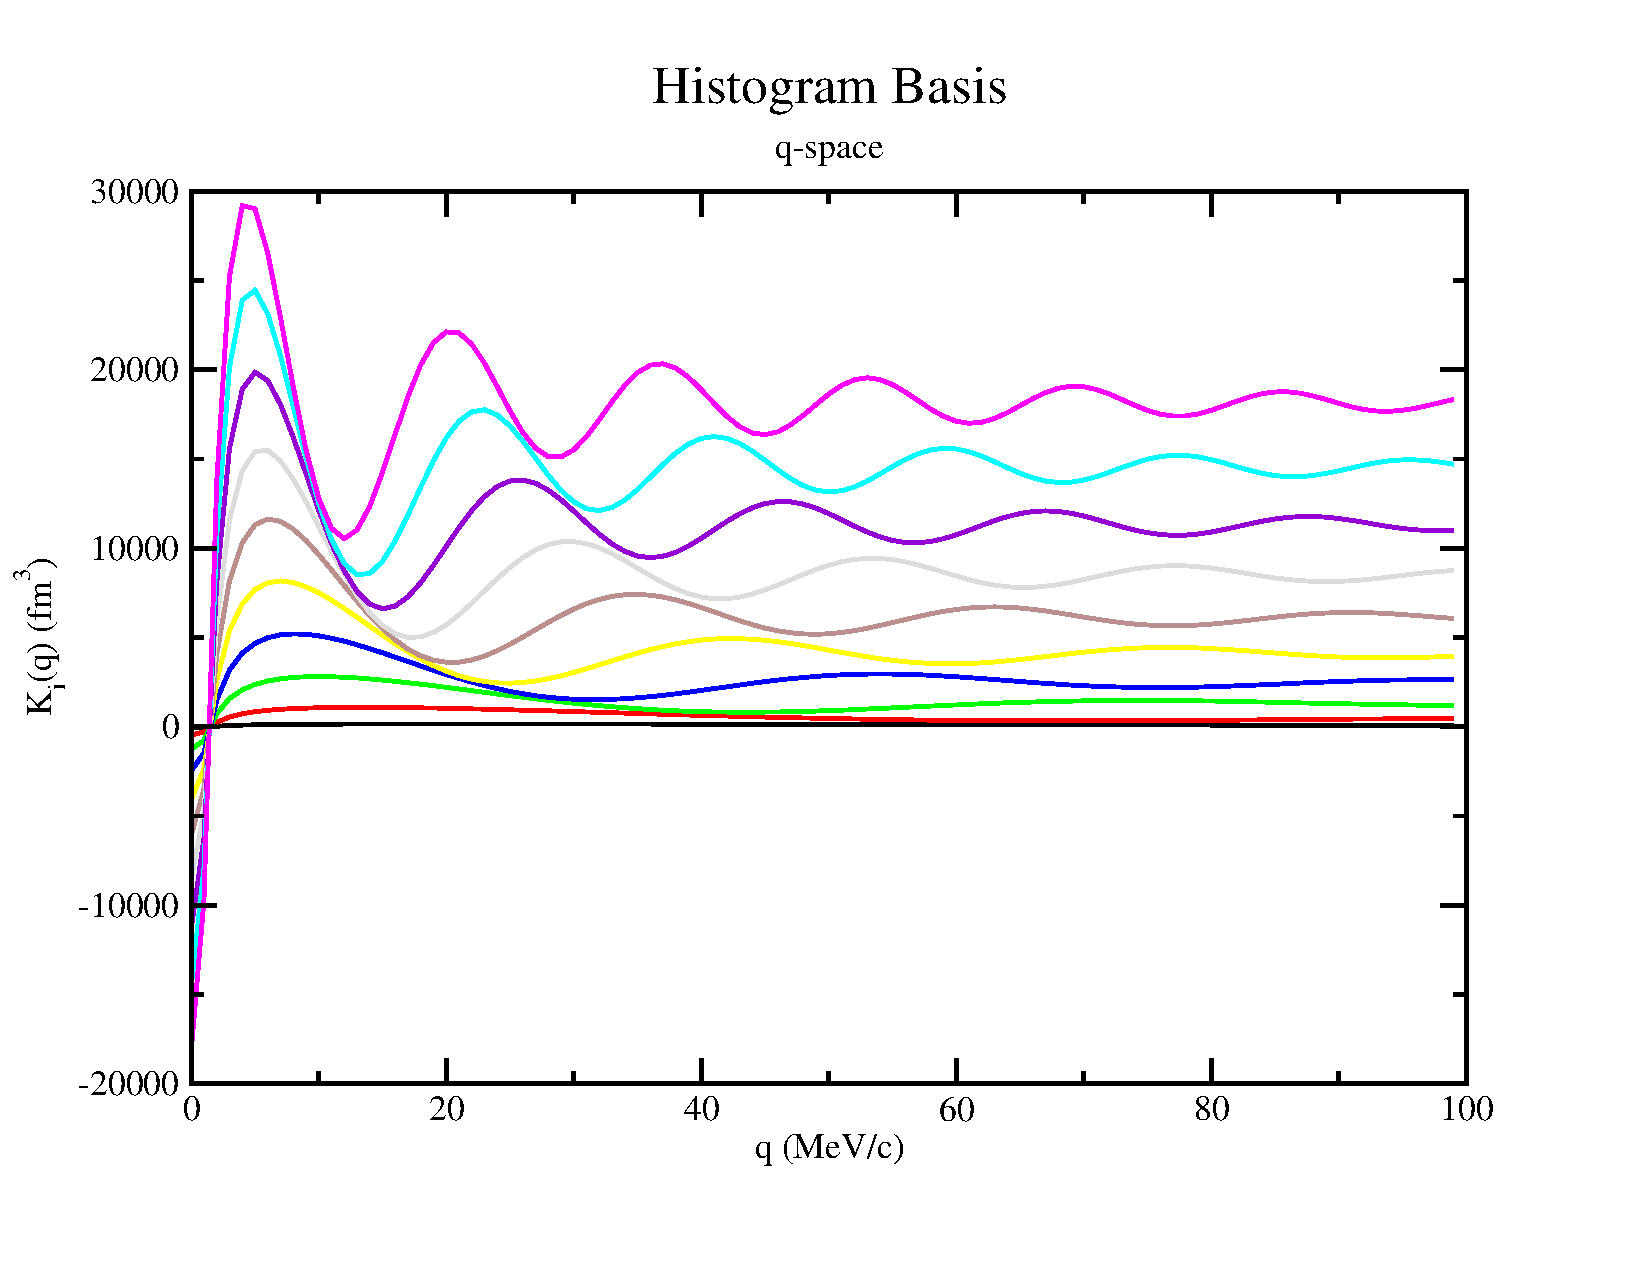
\includegraphics[width=0.47\textwidth]{basis_function_plots/Histogram_Basis_q}    
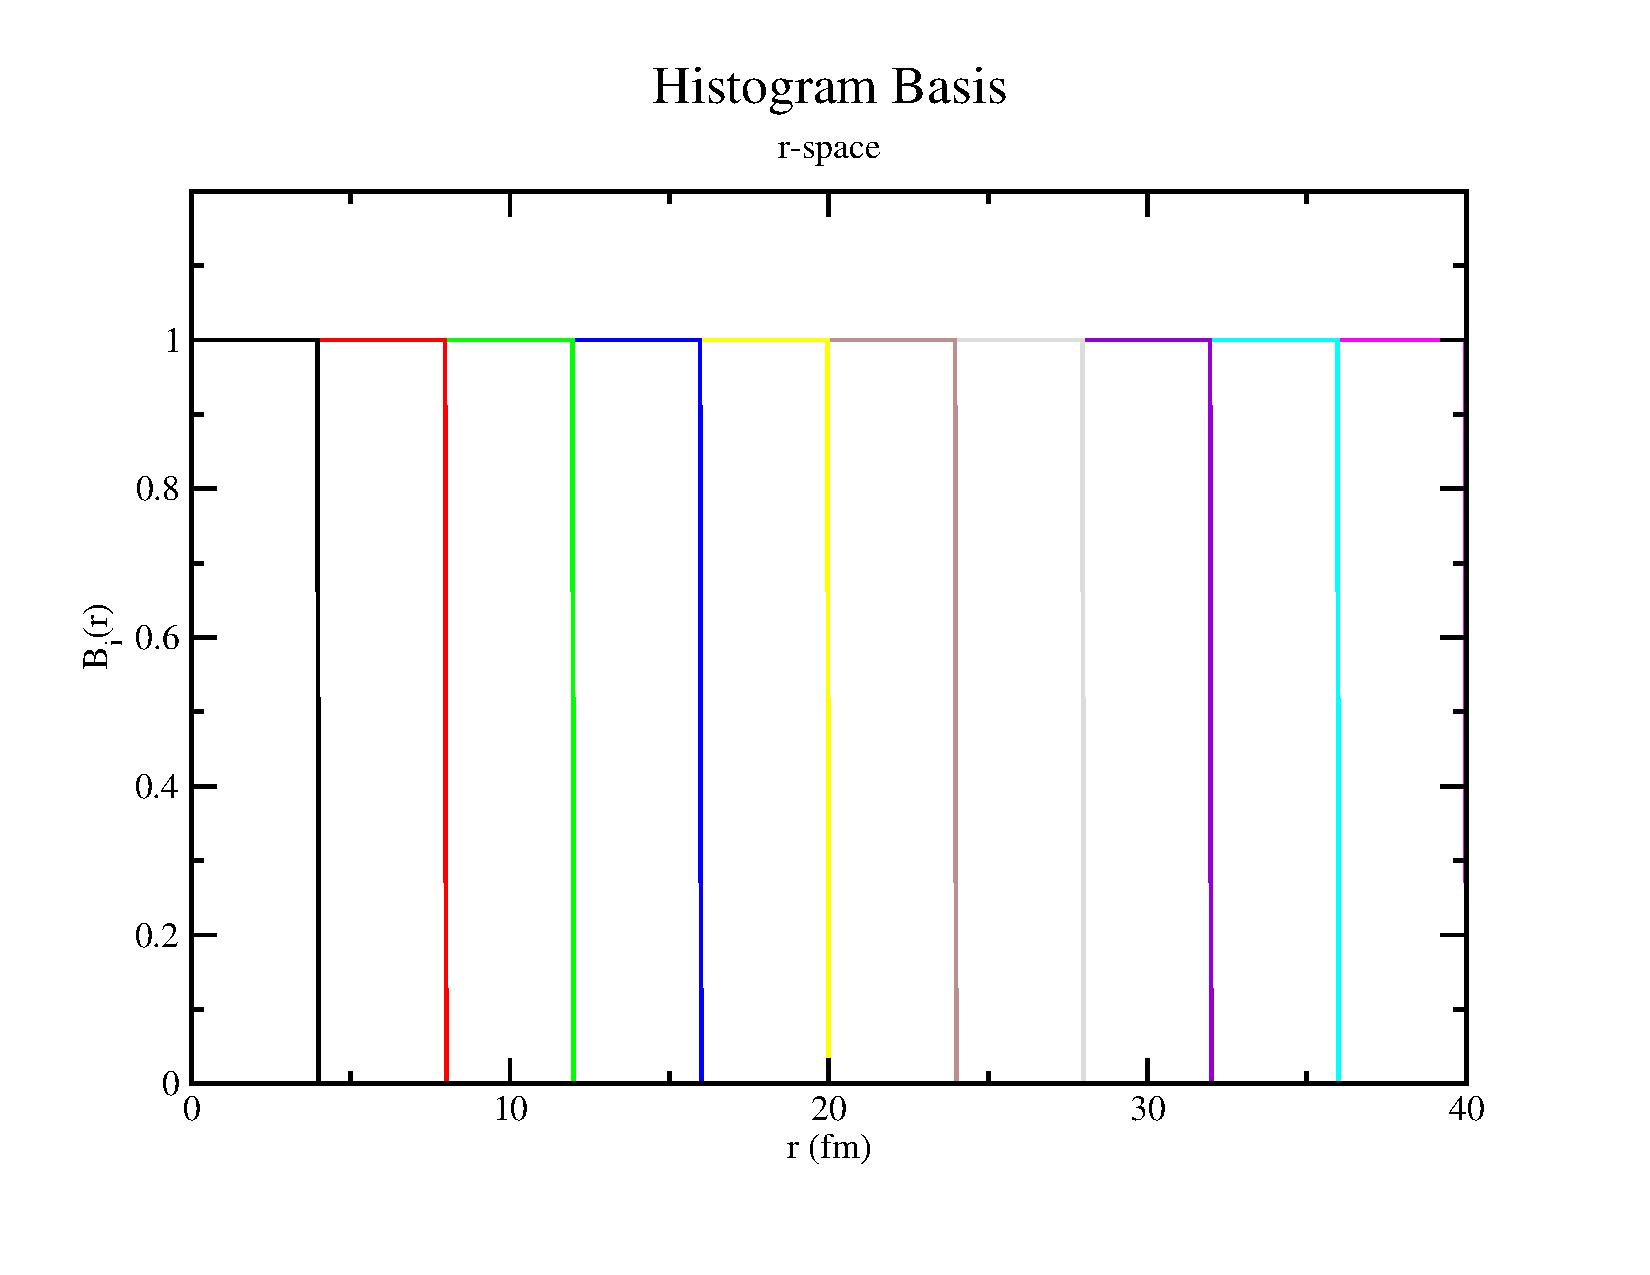
\includegraphics[width=0.47\textwidth]{basis_function_plots/Histogram_Basis_r}    
\end{tabular}    
\caption{\label{Histogram} Histogram basis}    
\end{figure*}

\begin{figure*}
\begin{tabular}{cc}        
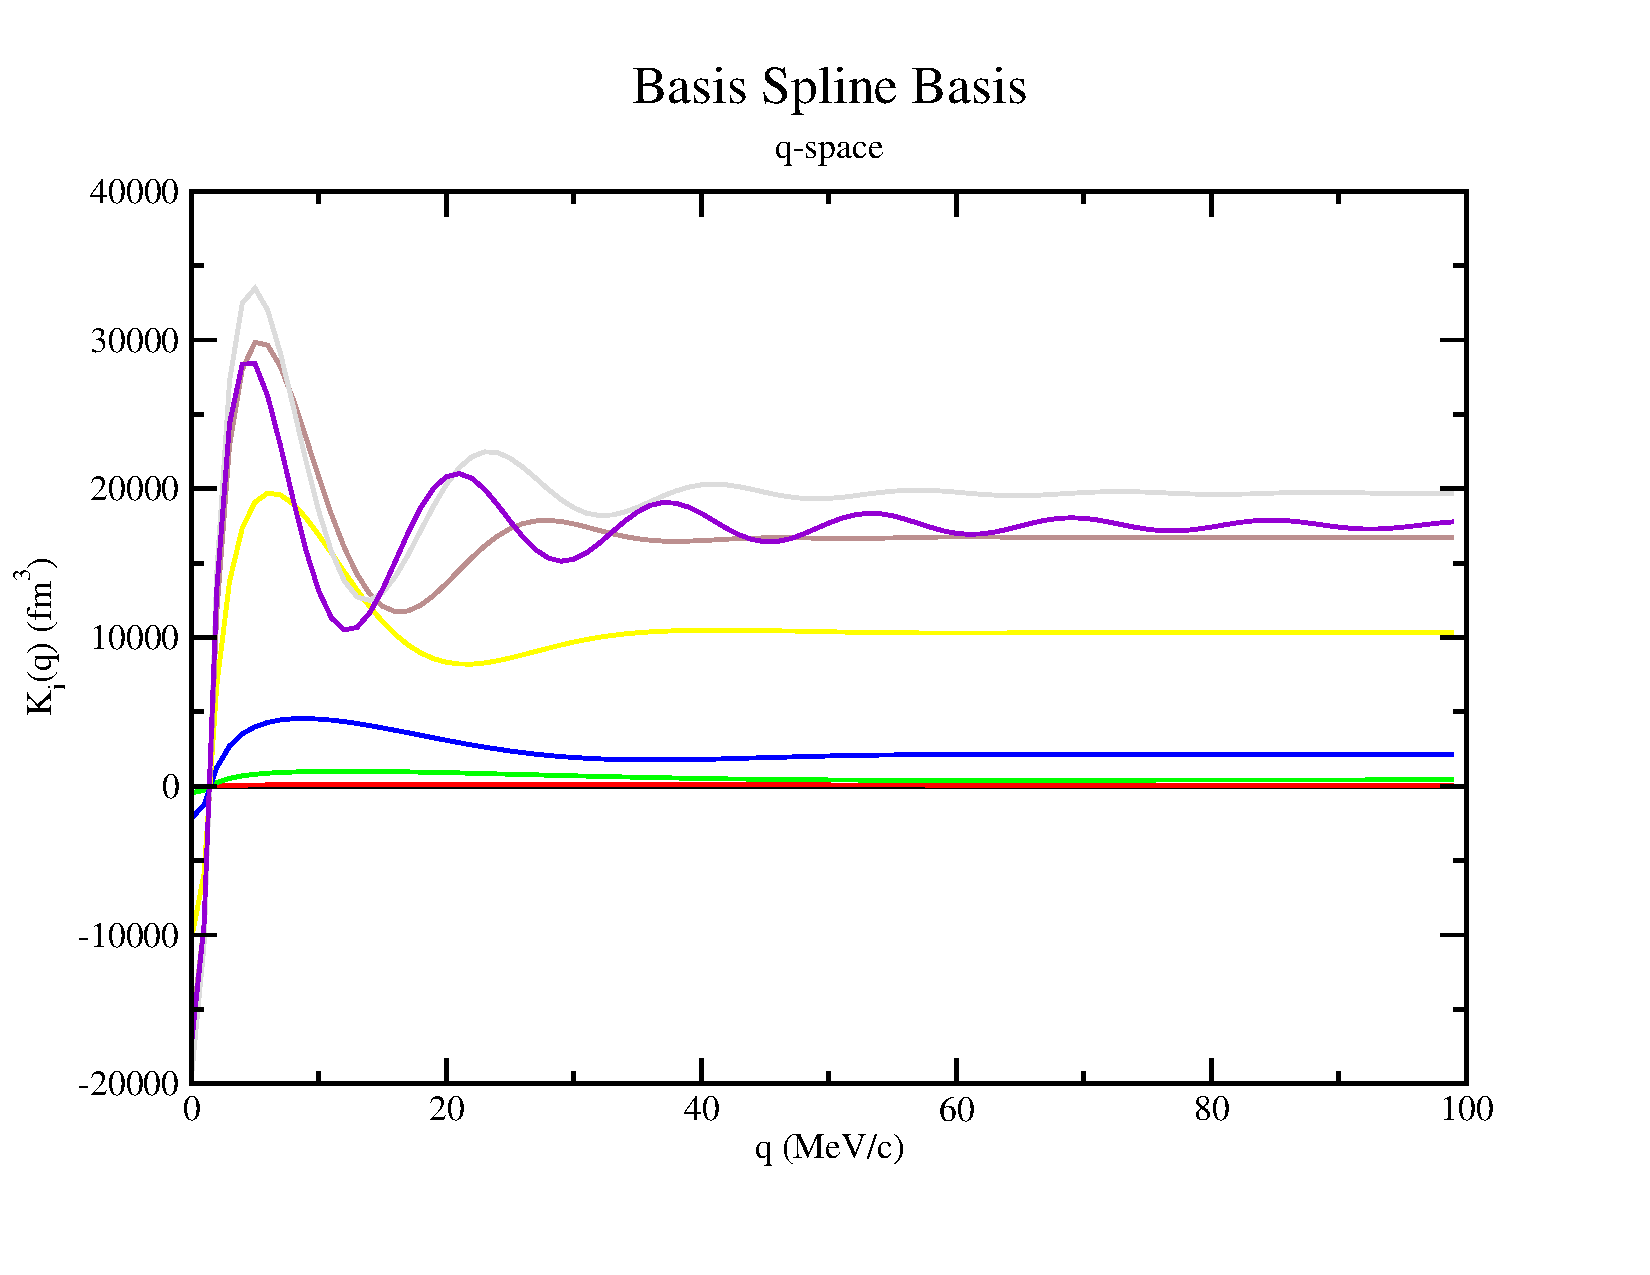
\includegraphics[width=0.47\textwidth]{basis_function_plots/BasisSpline_Basis_q}    
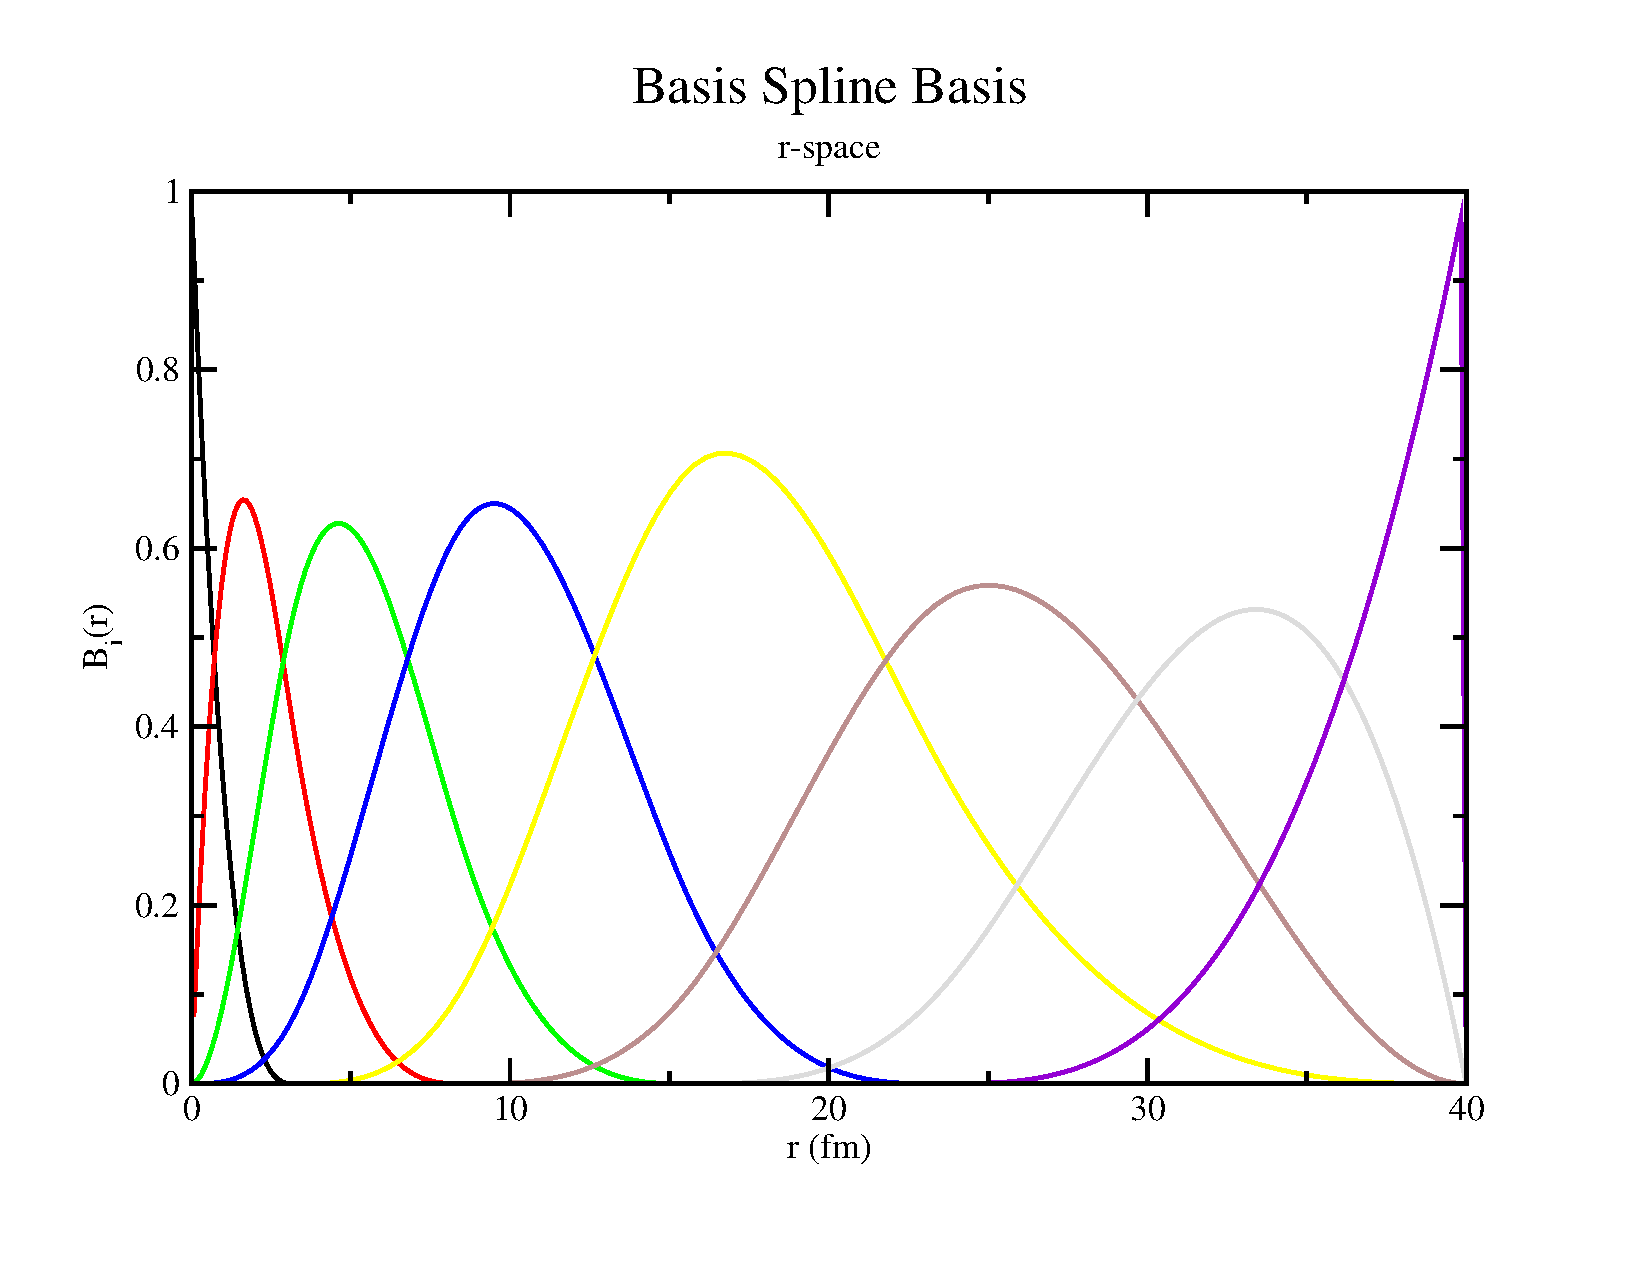
\includegraphics[width=0.47\textwidth]{basis_function_plots/BasisSpline_Basis_r}    
\end{tabular}    
\caption{\label{BasisSpline} Basis Spline Basis}    
\end{figure*}

\begin{figure*}
\begin{tabular}{cc}        
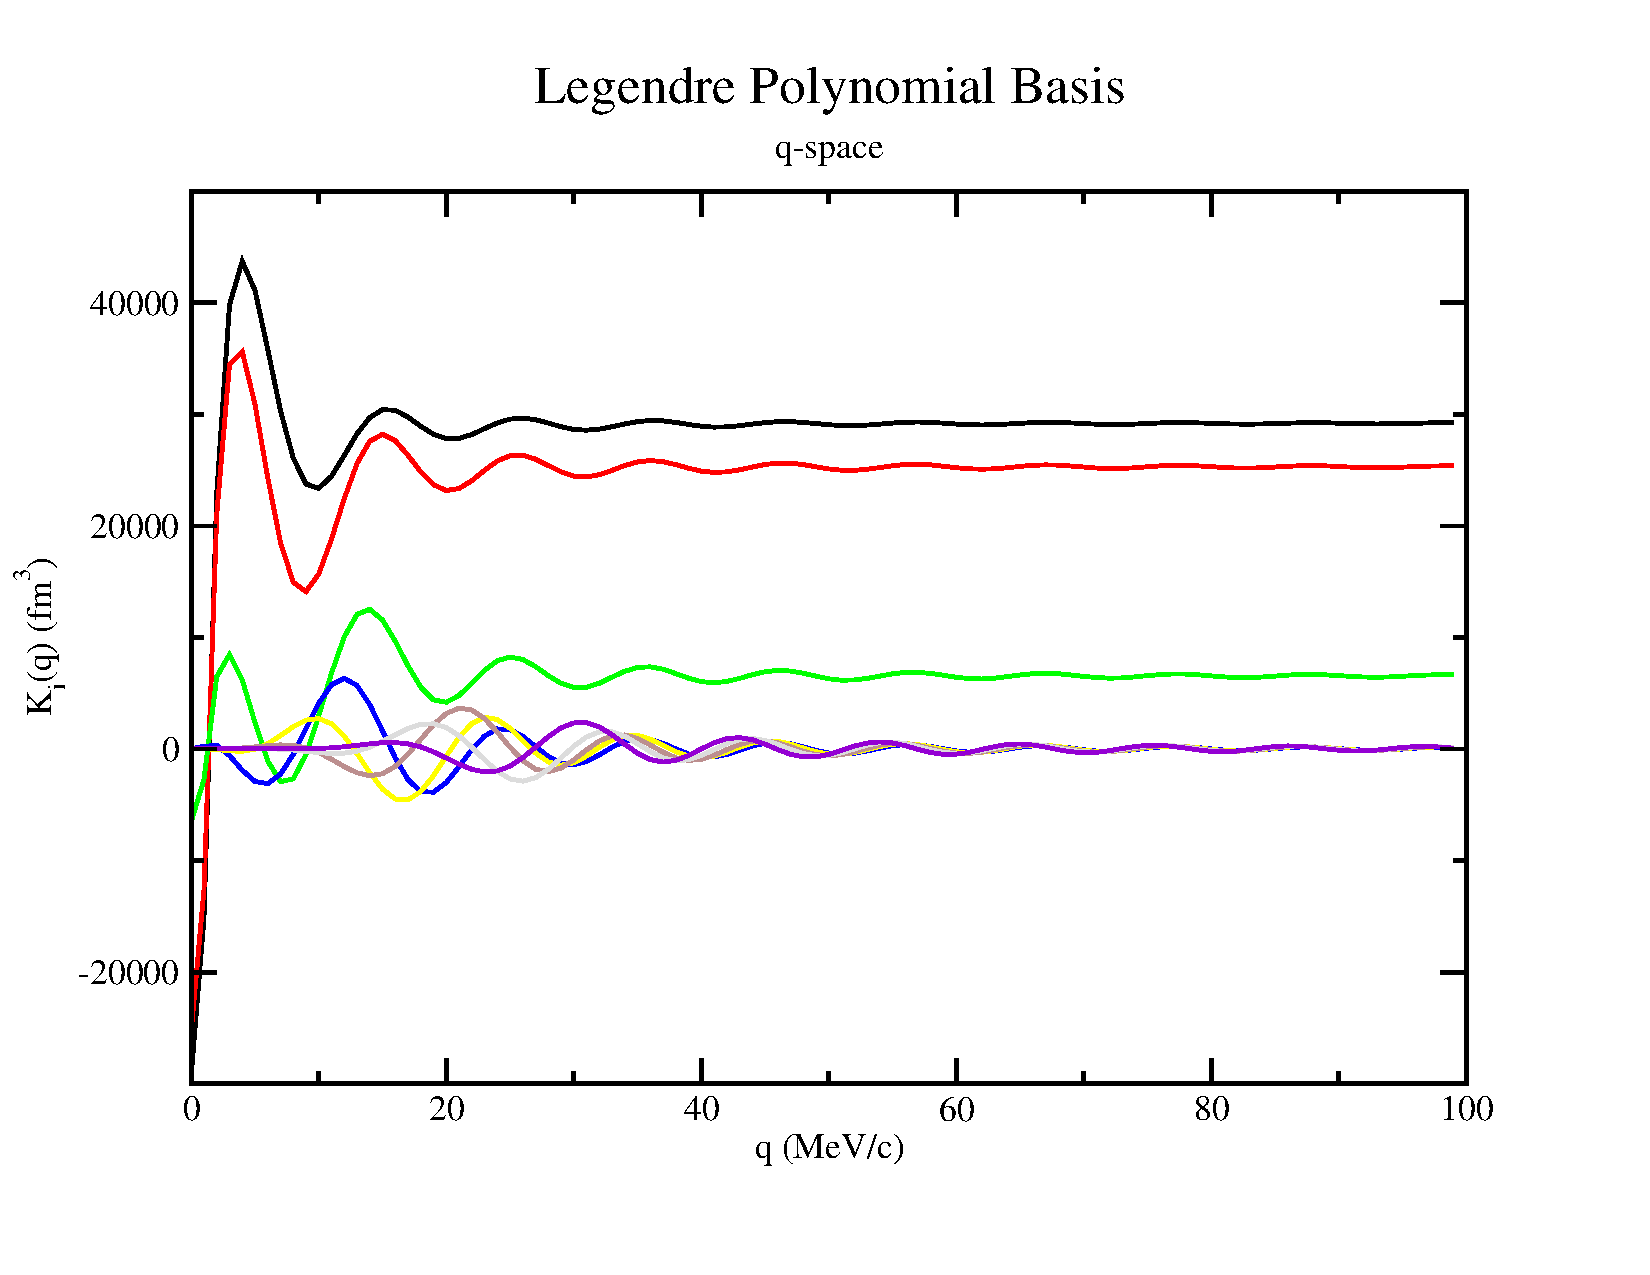
\includegraphics[width=0.47\textwidth]{basis_function_plots/Legendre_Basis_q}    
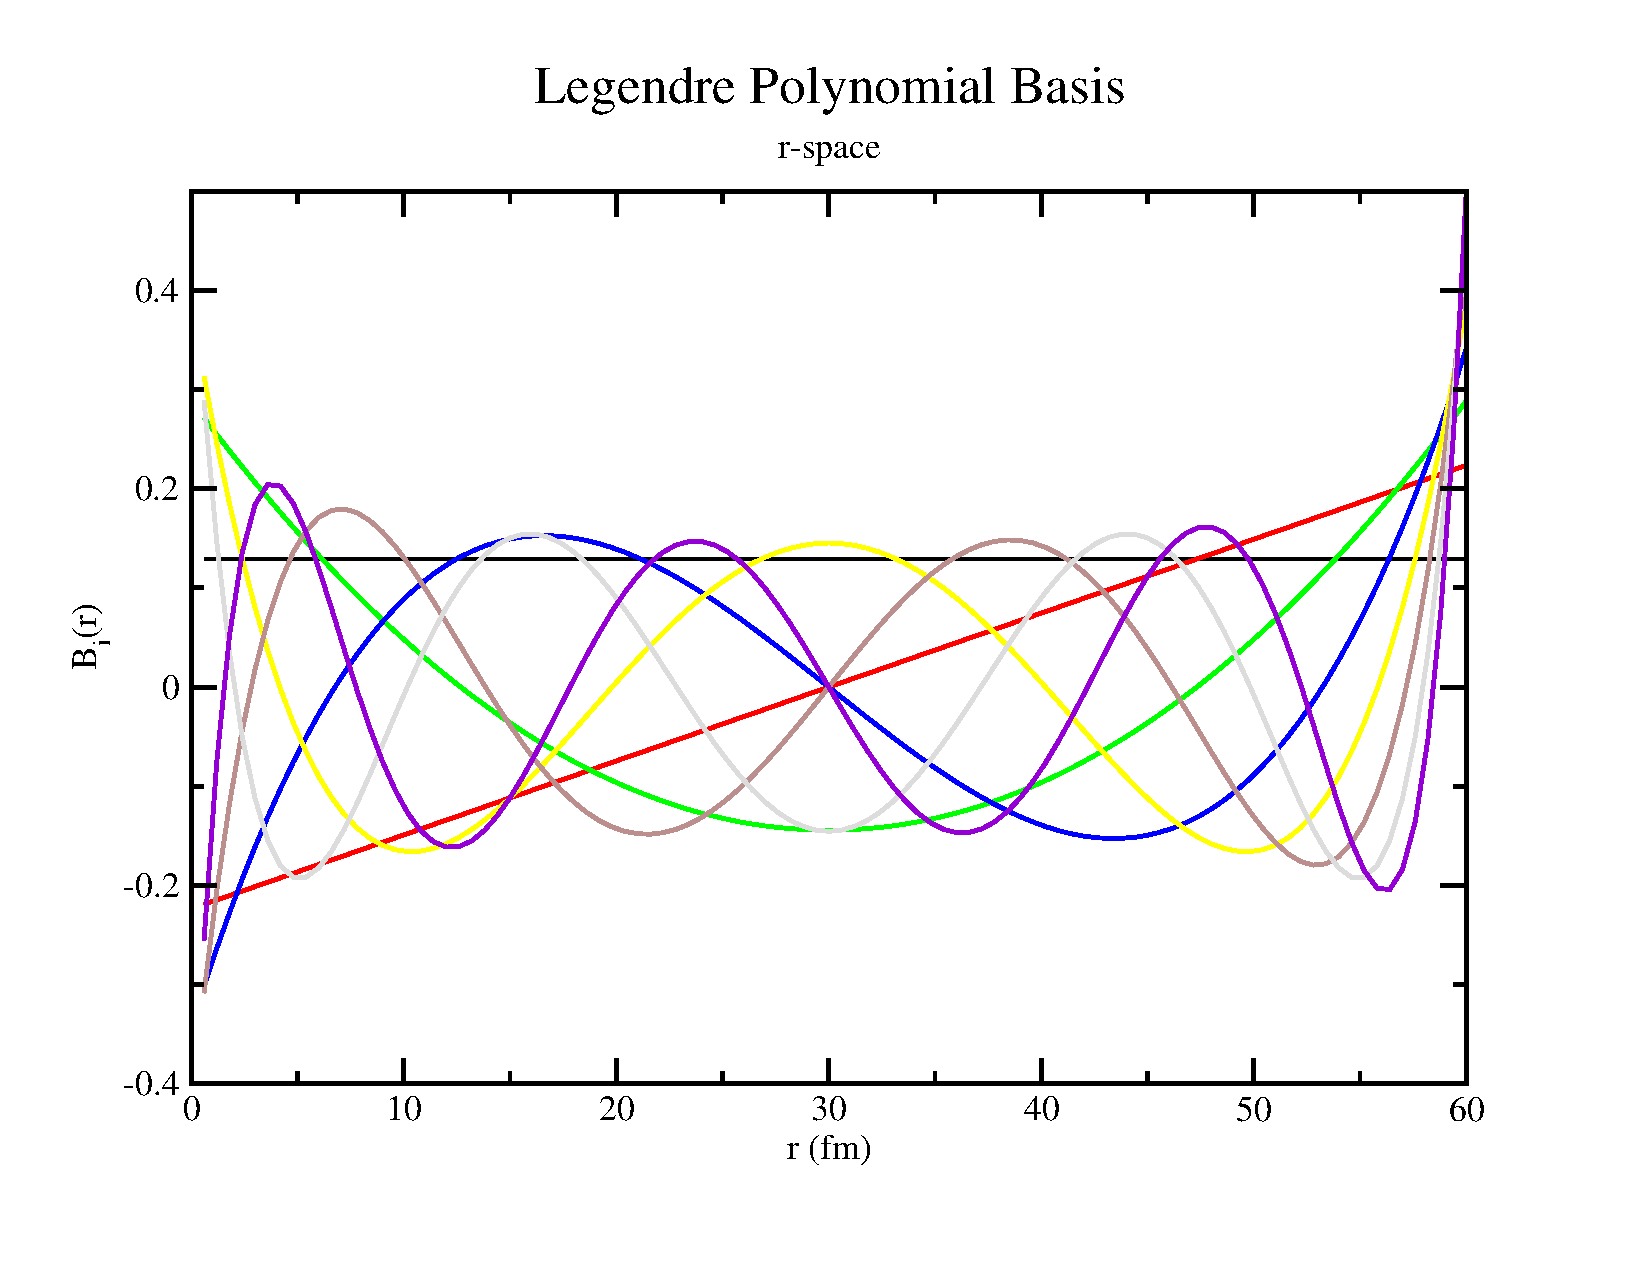
\includegraphics[width=0.47\textwidth]{basis_function_plots/Legendre_Basis_r}    
\end{tabular}    
\caption{\label{Legendre} Legendre Basis}    
\end{figure*}

\begin{figure*}
\begin{tabular}{cc}        
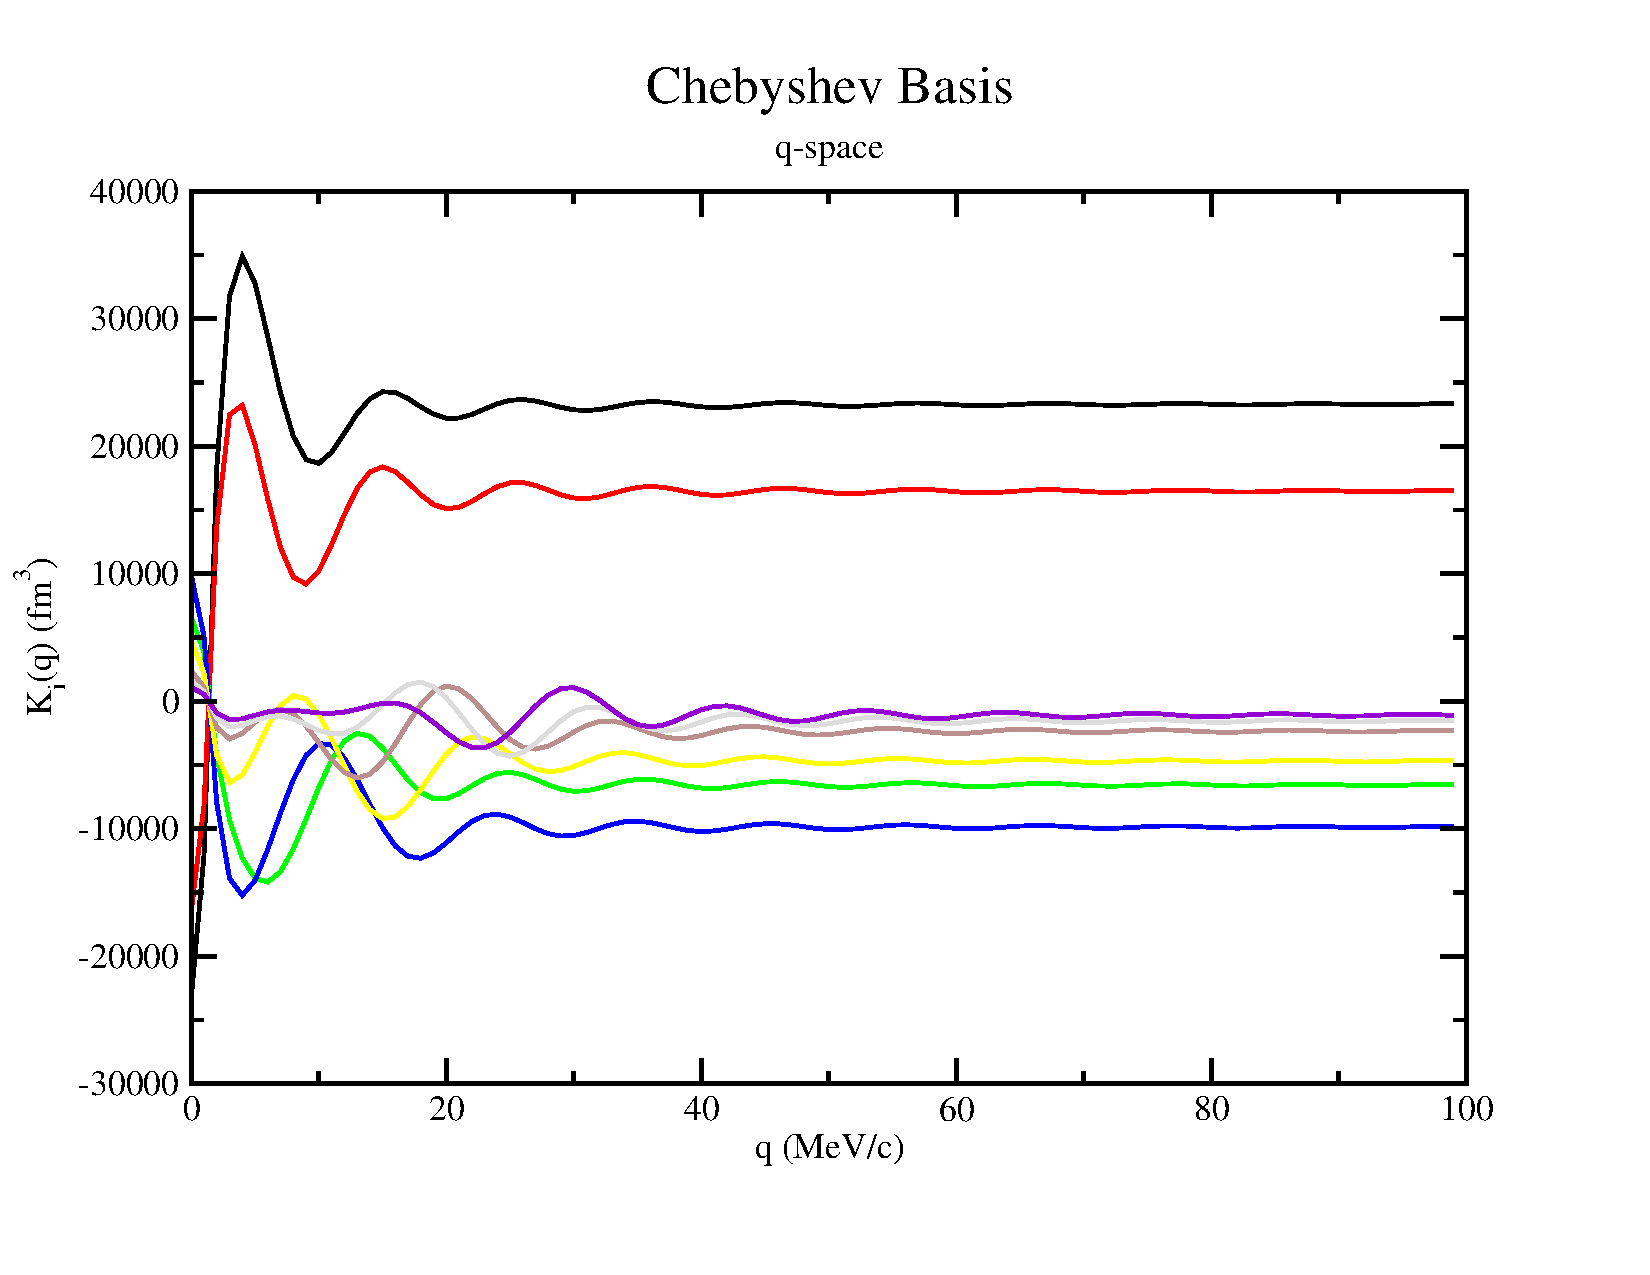
\includegraphics[width=0.47\textwidth]{basis_function_plots/Chebyshev_Basis_q}    
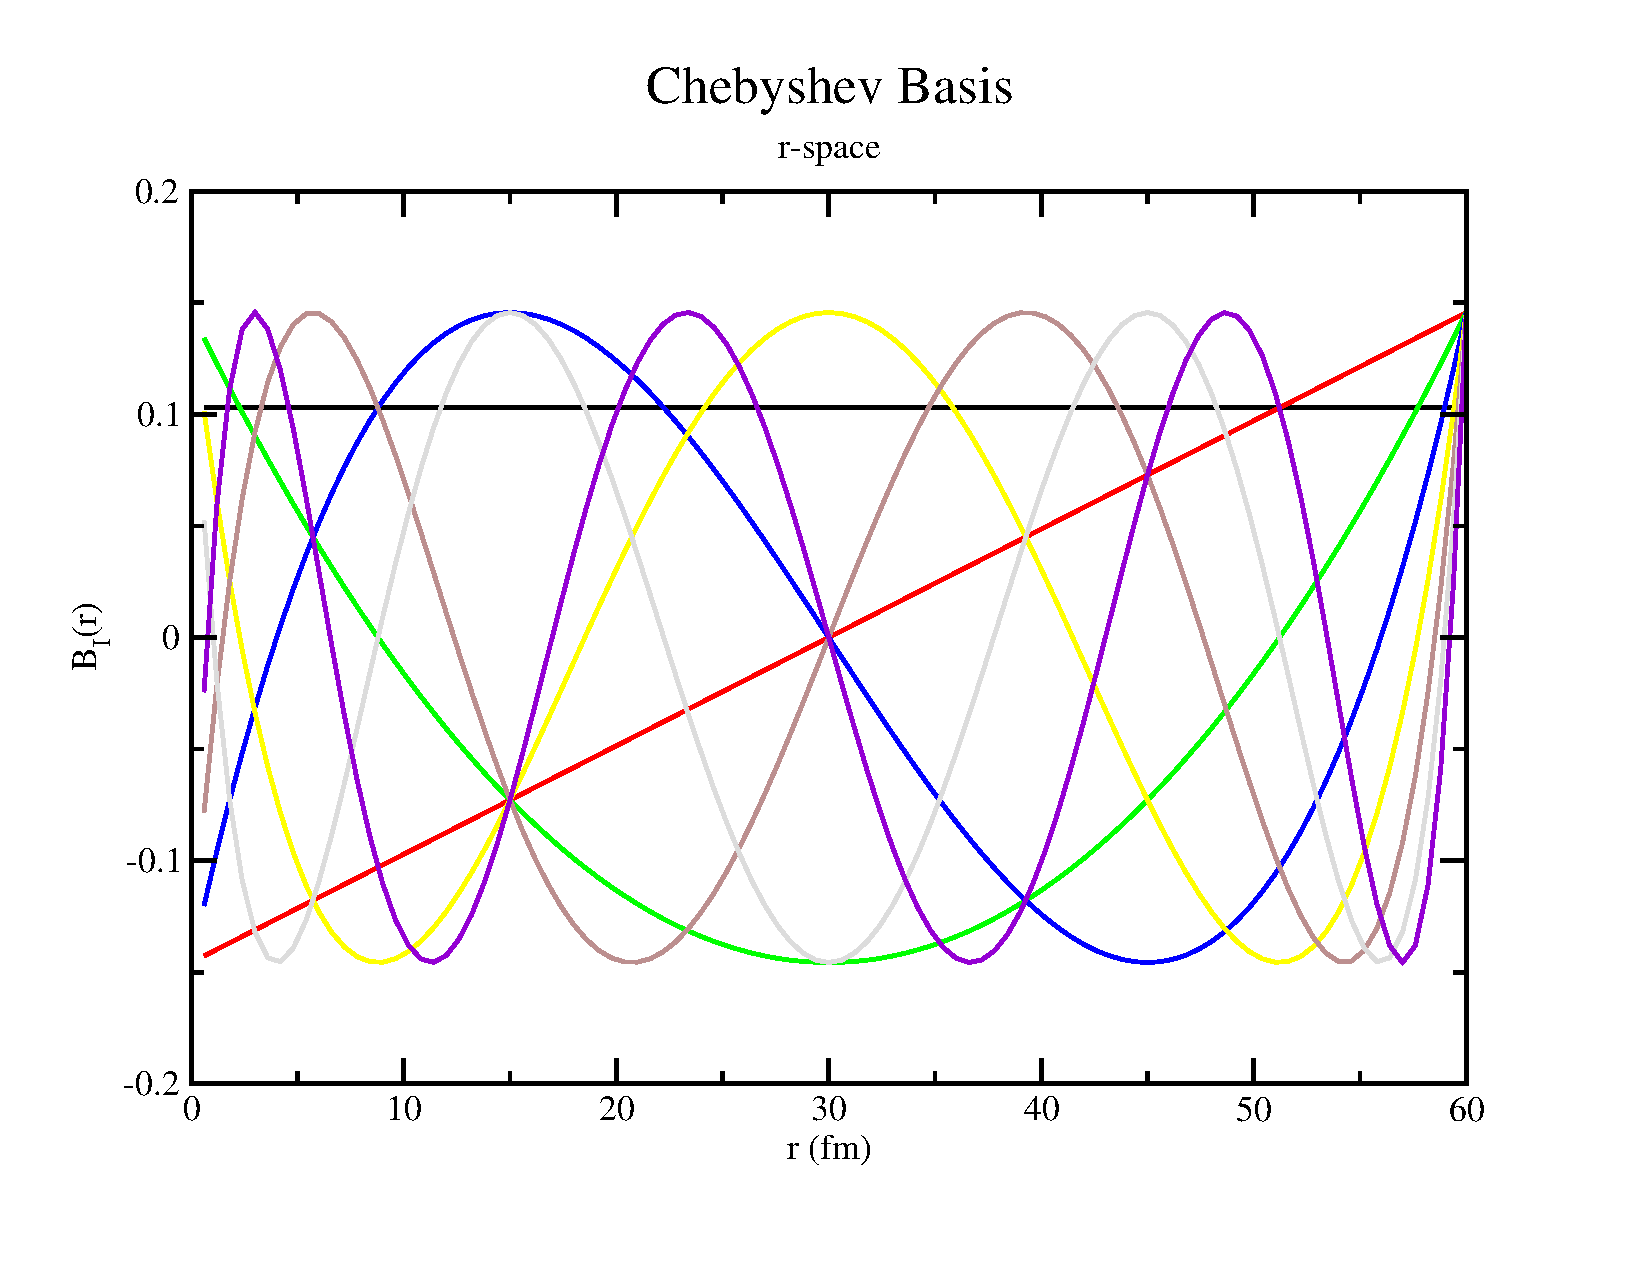
\includegraphics[width=0.47\textwidth]{basis_function_plots/Chebyshev_Basis_r}    
\end{tabular}    
\caption{\label{Chebyshev} Chebyshev Basis}    
\end{figure*}

\begin{figure*}
\begin{tabular}{cc}        
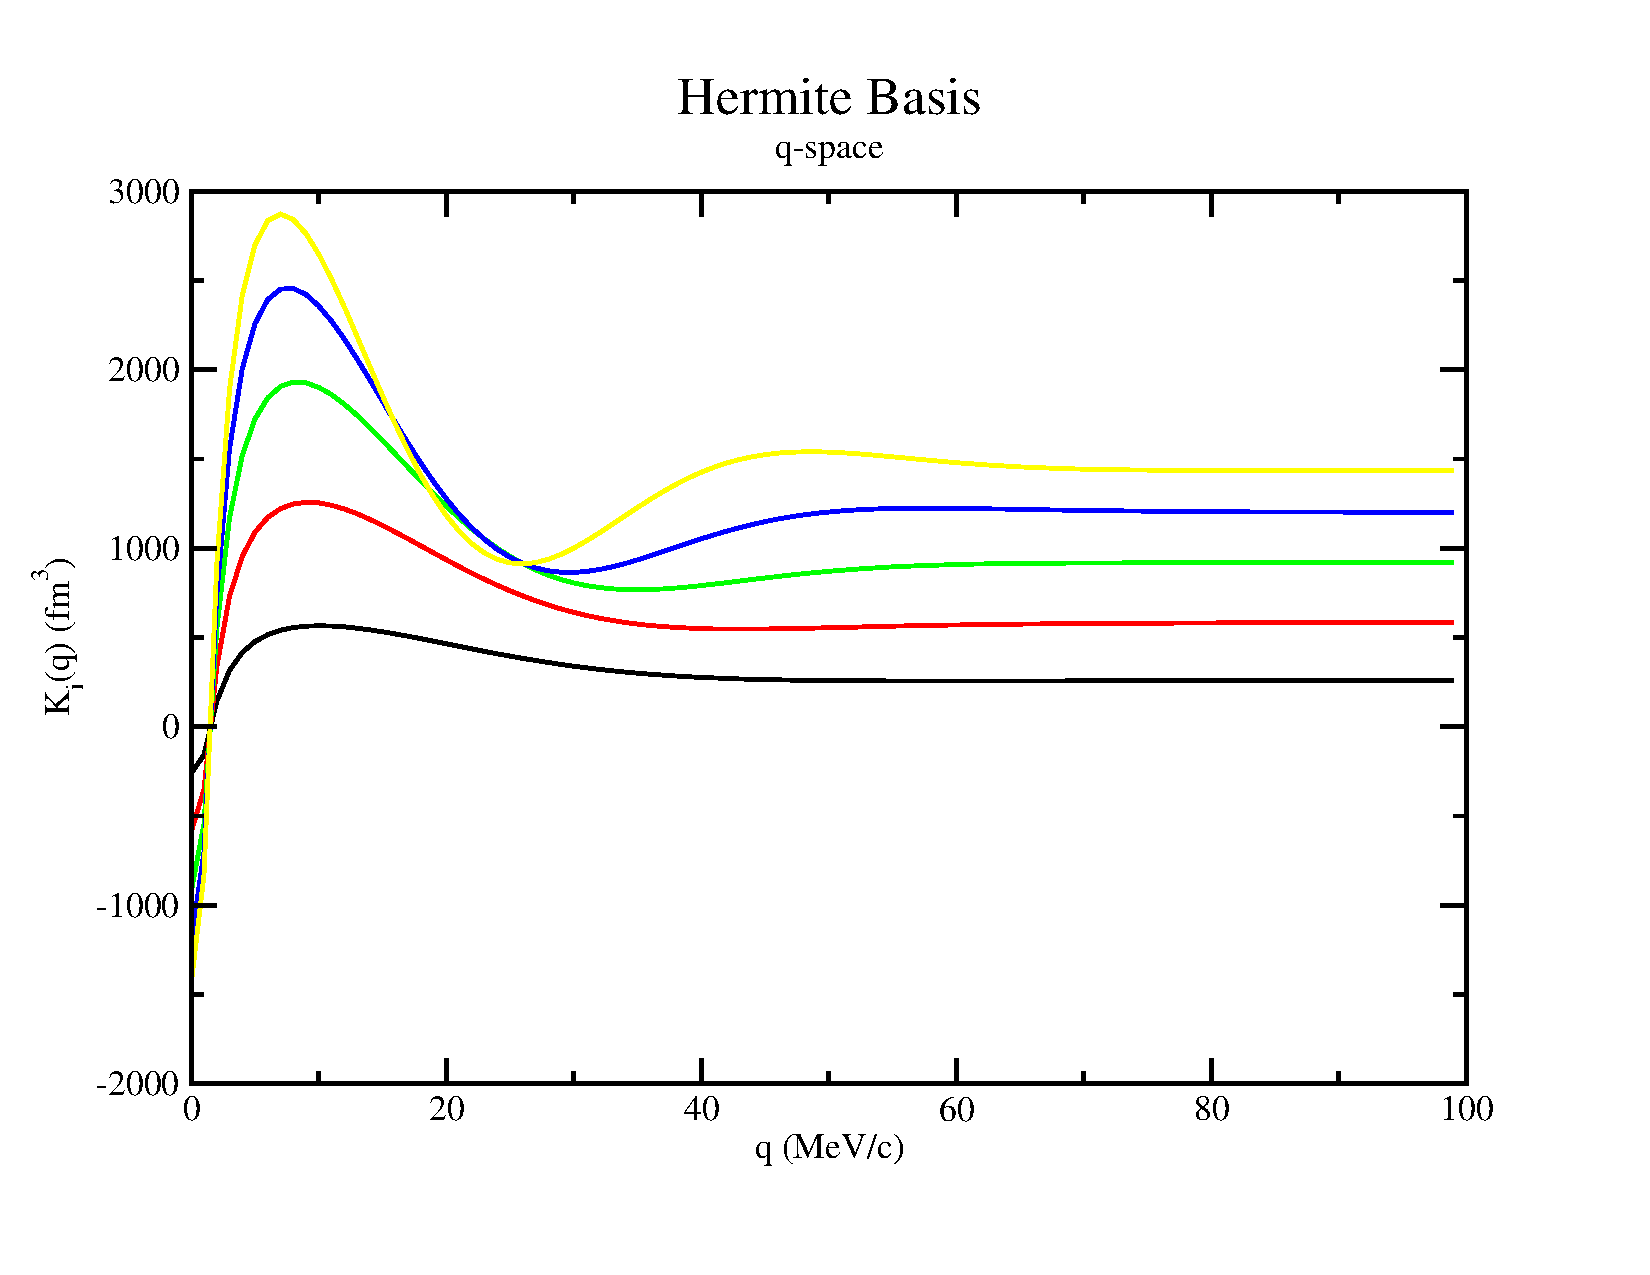
\includegraphics[width=0.47\textwidth]{basis_function_plots/Hermite_Basis_q}    
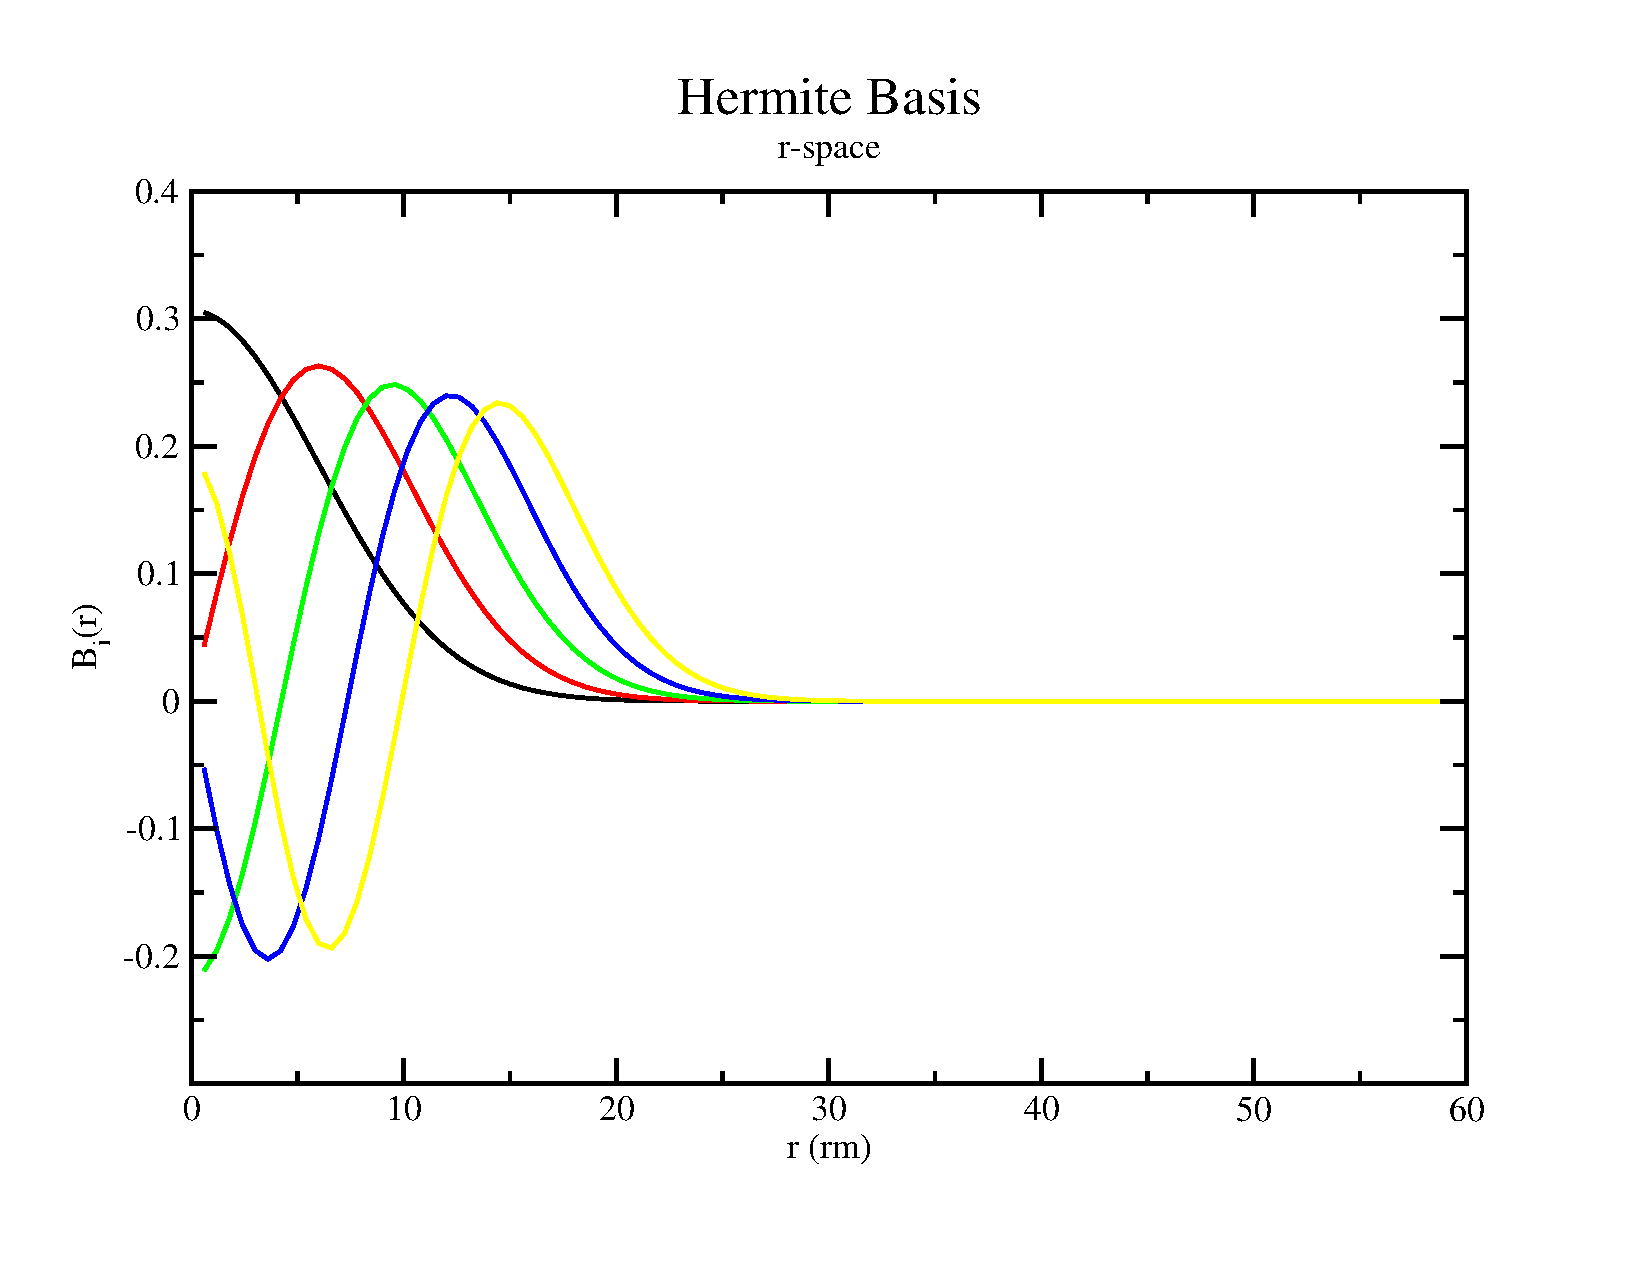
\includegraphics[width=0.47\textwidth]{basis_function_plots/Hermite_Basis_r}    
\end{tabular}    
\caption{\label{Hermite} Hermite Basis}    
\end{figure*}

\begin{figure*}
\begin{tabular}{cc}        
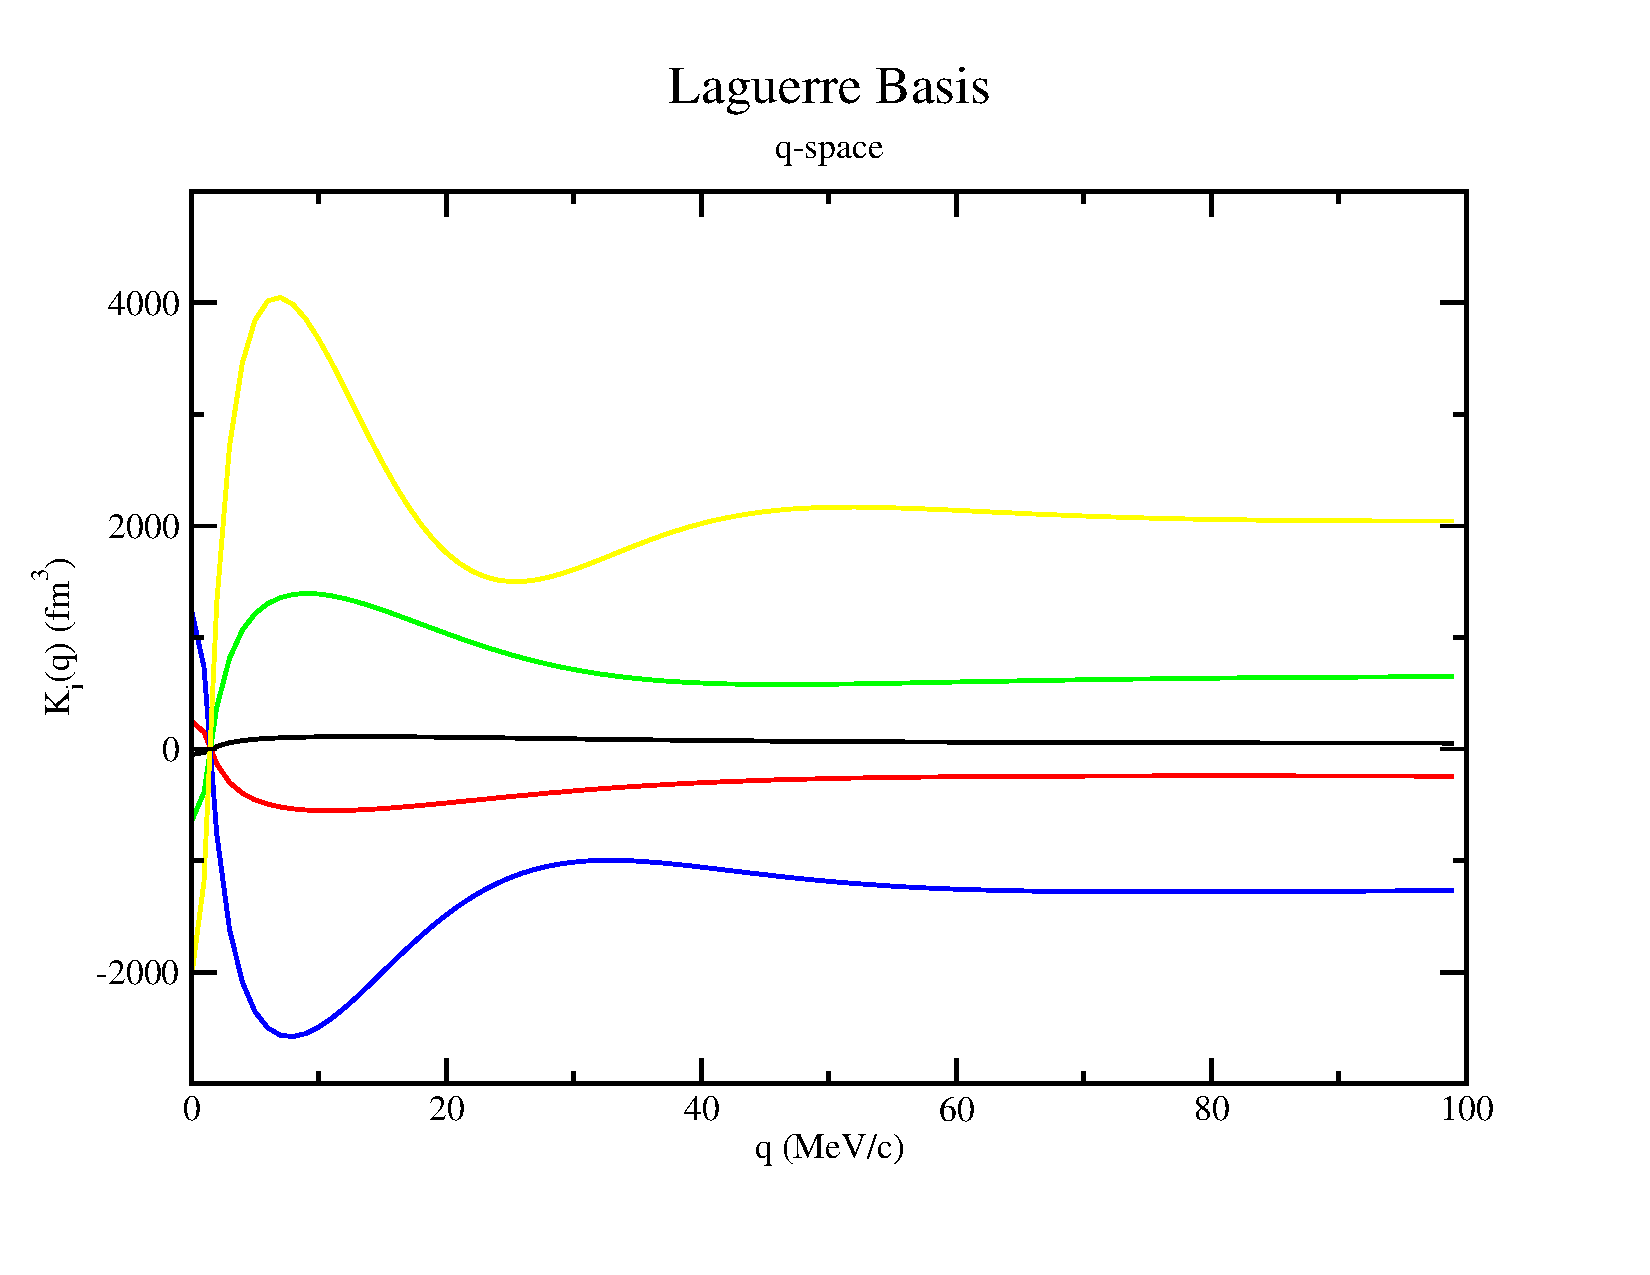
\includegraphics[width=0.47\textwidth]{basis_function_plots/Laguerre_Basis_q}    
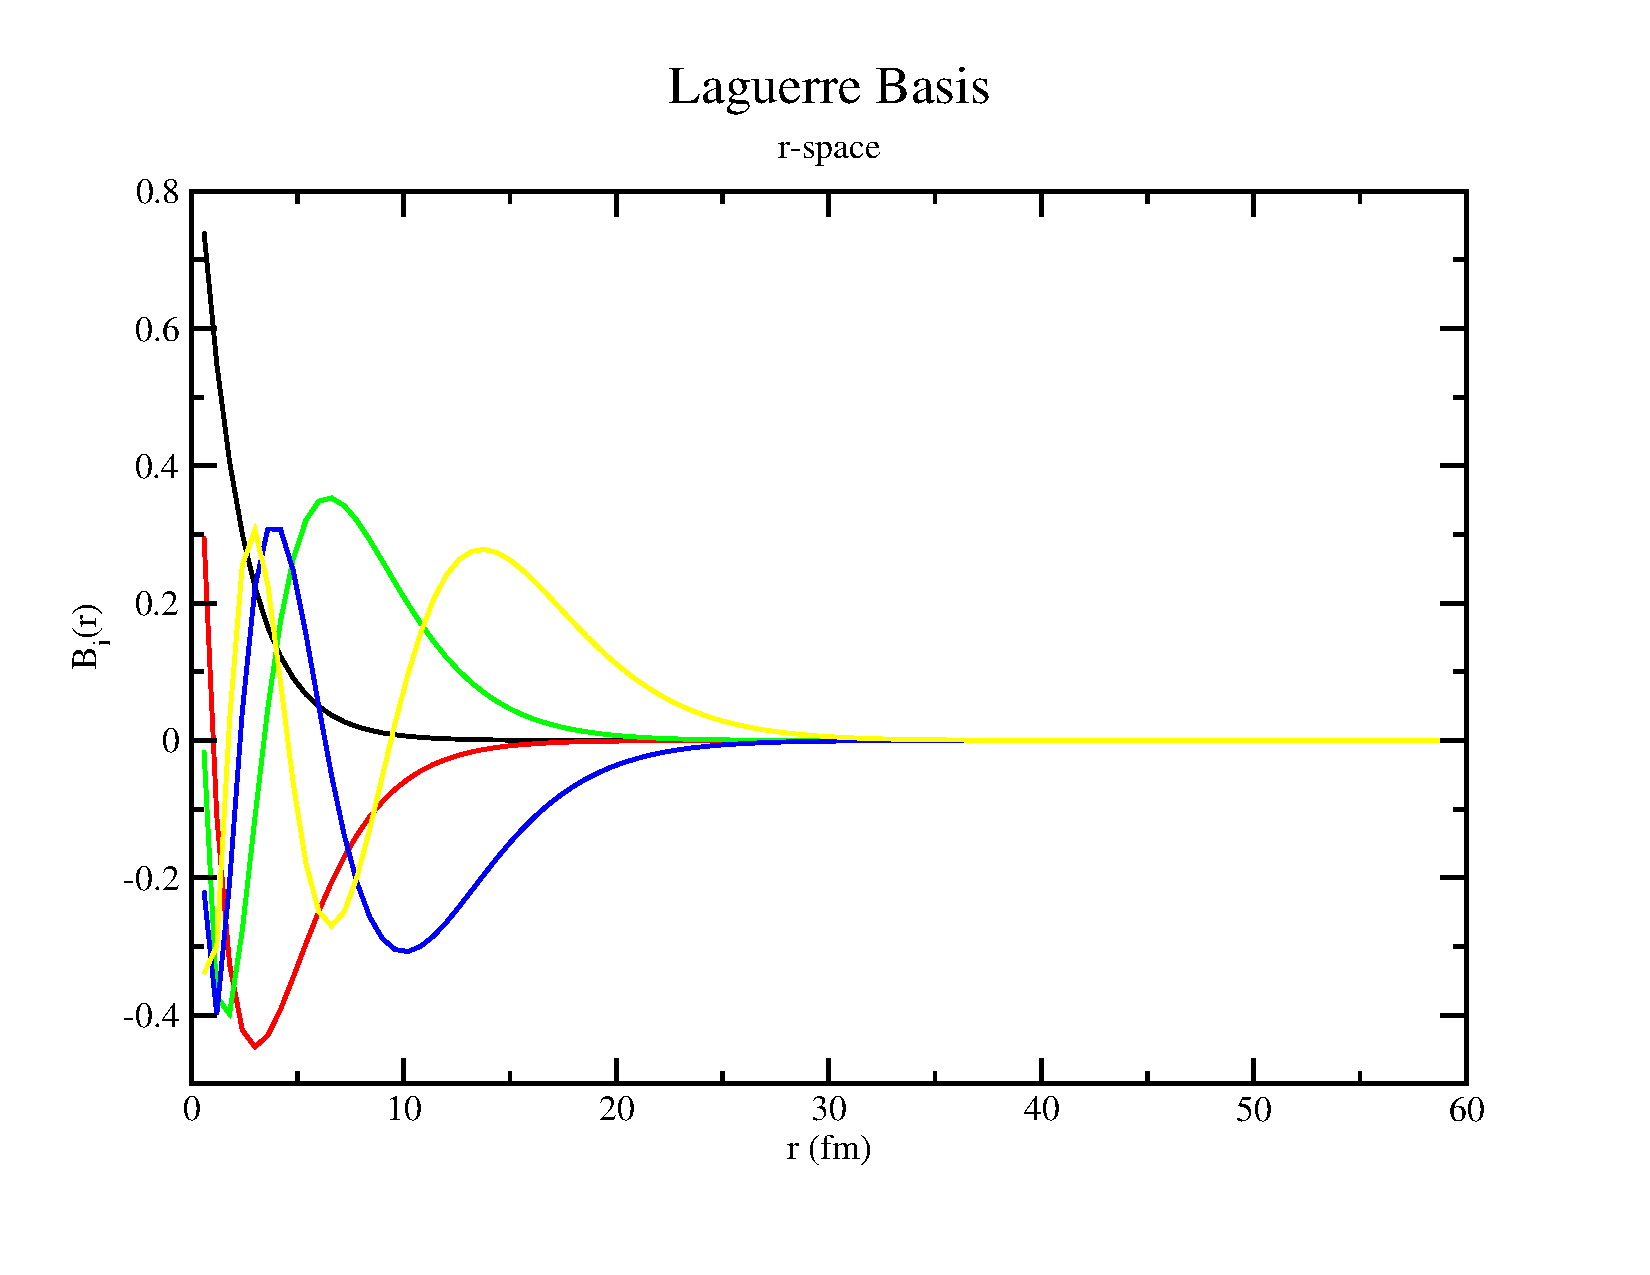
\includegraphics[width=0.47\textwidth]{basis_function_plots/Laguerre_Basis_r}    
\end{tabular}    
\caption{\label{Laguerre} Laguerre Basis}    
\end{figure*}

\section{Test Problem}
%% BEGIN MASSIVE PLAGARISM FROM THE SOURCE TAIL PAPER!!!! %%
We now outline the Core-Halo Ur-Model (\CHUM) code, based off the \CorAL\ library, to generate test data.  \CHUM\ is the simple variant of the Blast-Wave model used in Ref. \cite{srcTail}.              
The building blocks for our two-particle source are the normalized particle emission rates for the core and halo:
\begin{equation}
    D({\bf r}, t, {\bf p}) = fD_{\rm core}({\bf r}, t, {\bf p}) + (1-f)D_{\rm halo}({\bf r}, t, {\bf p})
\end{equation}
The core component (fraction = $f$), consists of a Gaussian spatial part, an exponential time profile, and a momentum dependence arising from hydro-like Boltzman factor:
\begin{equation}
    D_{\rm core}({\bf r}, t, {\bf p}) \propto e^{-p_{\mu} u^{\mu}/T -r^2_x/2R^2_x -r^2_y/2R^2_y -r^2_z/2R^2_z -t/\tau_{fo}}
\end{equation}
Here, $f$, $T$, $R_x$, $R_y$, $R_z$, and $\tau_{fo}$ are all adjustable and are specified in the lab frame.  For this study we set $T = 165$ MeV, $f=0.5$, $R_x = R_y \equiv R_T = R_z = 4$~fm, and $\tau_{fo}=10$~fm/c.  The flow profile is given by
\begin{equation}
    u_{\mu}(r) = \left(\cosh\eta \cosh\rho, \hat{r}_{T}\sinh\rho, \sinh\eta \cosh\rho\right)    
\end{equation}
where $\eta = \frac{1}{2}\ln\left(\frac{t+z}{t-z}\right)$ and $\rho = \rho_{0}r_{T}/R_{\rm max}$ with $\rho_{0}=0.6$.  These parameters were chosen arbitrarily since this paper is a generic study of the time profile and $\omega$ contributions to the source distribution.  Indeed, we have experimented with other flow profiles and found no significant differences.  For comparison, the Blast-Wave fits of Retiere and Lisa~\cite{blastwave} for central collisions converged for $R_x \approx R_y \approx 13$~fm (equivalent to a 2D rms Gaussian radius of 6.5~fm), $T \approx 110$~MeV, and $\rho_{0} \approx 0.9$. 

Following earlier work on the contribution of resonance decays to the pion source distribution~\cite{Wiedemann:1996ig,Sullivan93}, we assume that the halo is dominated by the decay of the $\omega$ resonance ($\tau_\omega = 23$ fm/c), with a fractional contribution of 50\% to the pion distribution in the region of $0.2<k_T<0.36$~GeV. Other potential candidate resonances have decay times that are much too short, e.g. the $\rho$ with lifetime $\tau_\rho = 1.3$ fm/c, or too long, e.g. the $\eta'$ with lifetime $\tau_{\eta'} = 975$ fm/c or have charged pionic decay modes with small branching fractions.  The $\omega$'s are emitted from the same core, but we allow them to propagate classically for some distance before decaying into pions:
\begin{equation}
\begin{array}{rl}
    D_{\rm halo}({\bf r}, t, {\bf p}) \propto &\displaystyle\int \dn{}{\Delta t} \dn{3}{p_\omega} P({\bf p}_\omega, {\bf
p}) e^{-\Delta t/\tau_{\omega}} \\
&\displaystyle \times D_{\rm core}({\bf r}-\frac{{\bf p}_\omega}{E_\omega}\Delta t, t-\Delta t, {\bf p_\omega}).
\end{array}
\end{equation}
We include the dominant three-body reaction $\omega\rightarrow\pi^+\pi^-\pi^0$ with a branching fraction of 88.8\% and define the probability, $P$, for finding a $\pi$ with momentum ${\bf p}$ from the decay of the $\omega$ with momentum ${\bf p_\omega}$, using standard three-body decay kinematics.   We neglect the only other charged pion decay mode of the $\omega$ which is $\omega\rightarrow\pi^+\pi^-$ with a branching fraction of 2.2\%.  This mode would only have a negligible impact on the source distribution.

This source function is the probability to emit a pair with a separation of ${\bf r}'$ in the Pair Center of Mass System (PCMS) and is given by~\cite{imag1}
\begin{equation}
   S_{\bf P}({\bf r'})=\int \dn{}{r_0'} \int \dn{4}{R} D_1(R+r/2,{\bf P}/2) D_2(R-r/2,{\bf P}/2).
\label{eqn:sou-def}
\end{equation}
Here $r_{0}' = \gamma(r_{0}-\boldmath{\beta}\cdot{\bf r})$ is the relative time separation in the PCMS.  So, the integral over $r_{0}'$ serves to mix the time and space dependence of the emission functions in the lab frame into the space dependence of the source function in the PCMS.    

We construct the source function from the single particle source by Monte-Carlo integrating our emission function in Eq.~(\ref{eqn:sou-def}).  We work in Bertsch-Pratt coordinates \cite{pratt_90}, so that the time integral in Eq. (\ref{eqn:sou-def}) actually moves the time effects into a direction parallel to the boost velocity, $\boldmath \beta$, namely into the outward and longitudinal directions.  To compare to the 1D, angle-averaged source image for central Au-Au collisions recently measured by PHENIX~\cite{ppg052}, we keep only pairs where both pions have a pseudo-rapidity $|\eta|<0.35$ and transverse momentum $0.2$ $< k_{T} < 0.36$ GeV.  Because these acceptance cuts change the average pair boost from the lab to the PCMS, they can have a noticeable affect on the final source.  However, the STAR acceptance cuts in pseudo-rapidity, $|\eta|<0.5$, are close enough to those of PHENIX that we see no qualitative difference.
%% END MASSIVE PLAGARISM FROM THE SOURCE TAIL PAPER!!!! %%

To build the source function, we use the \CorAL\ re-implementation of the venerable CoRrelation AfterBurner (\CRAB) code.  \CRAB\ can generate both the source functions and correlation functions in either a Cartesian basis or in spherical harmonics.  Appendix \ref{buildFromPairs} describes how \CRAB\ does the weighted binning to construct the sources or correlations in detail.  Fig. \ref{srcTail} shows plots of the source function generated in a Cartesian representation and in spherical harmonic expansions of maximum various orders.  Here, $10^{8}$ pion pairs were used to generate the sources.  We comment that, with only 650 bins to determine at $\ell_{max} = 4$, the spherical harmonic representation is much better determined than the Cartesian histogram with $50^{3} = 12500$ bins.           

\begin{figure}
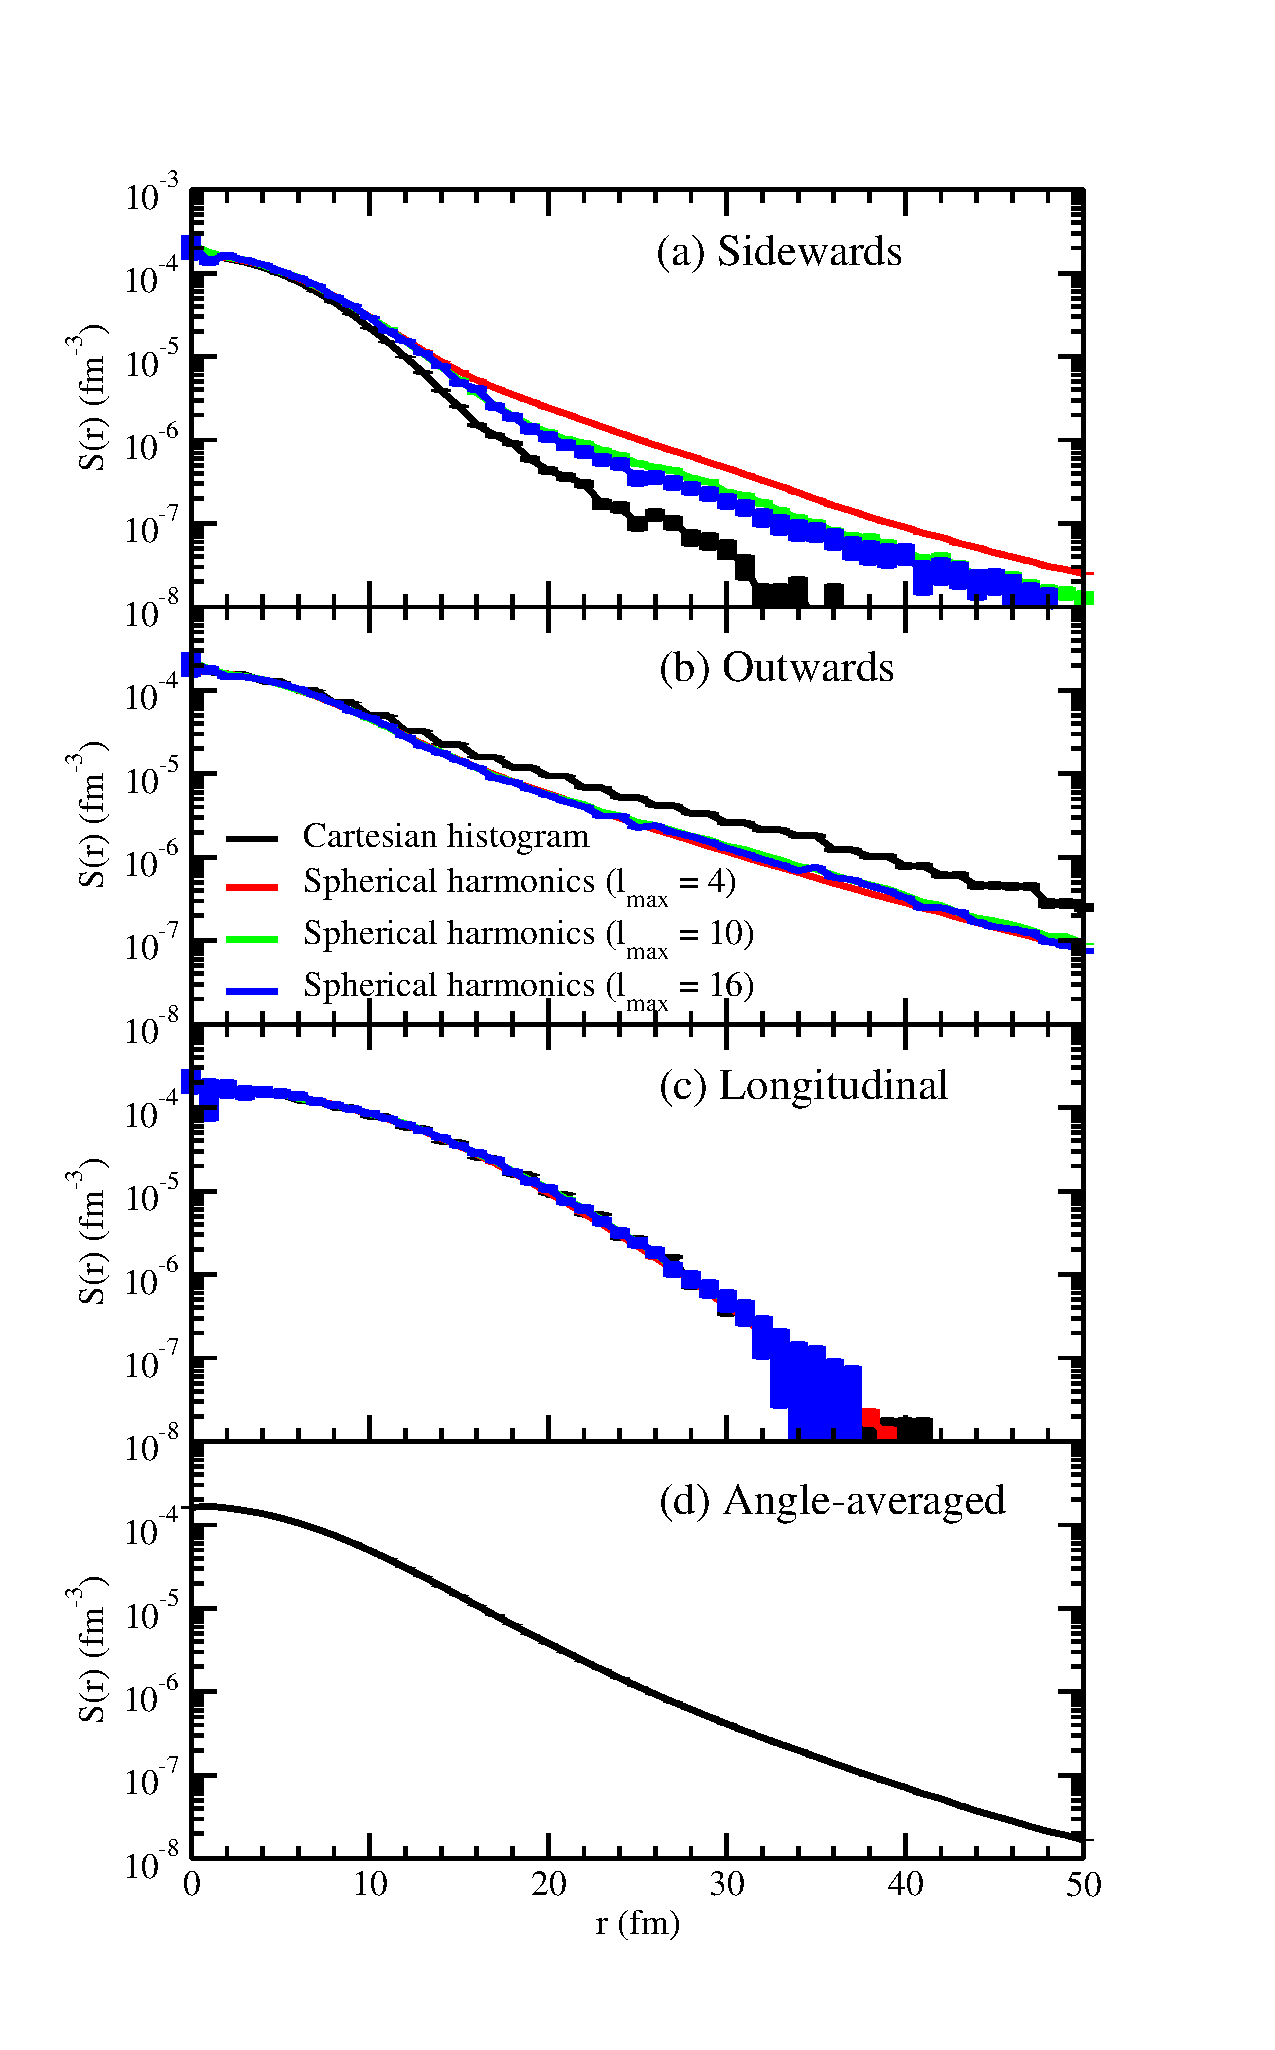
\includegraphics[width=0.47\textwidth]{chum_source_4panel}    
\caption{\label{srcTail} Plots of the test source function binned in Cartesian coordinates and in spherical harmonics.  The 3d histogram in Cartesian coordinates is not as well determined as the spherical harmonic expansion as described in the appendix.}    
\end{figure}

Using \CRAB, we can also compute the correlation  function directly in Spherical Harmonics.  In Fig. \ref{corrTailSlice}, we show the slices of the correlation  we obtain folding our test source with a non-interacting like-pion kernel, a $\pi^{+}\pi^{+}$  and a $K^{+}K^{+}$ kernel.   Since we will be imaging the spherical harmonic expanded correlation, we show plots of the various terms, using all three kernels, in the correlations in Fig. \ref{corrTailTerm}.  We comment that \CorAL\ has a variety of other kernels implemented (including most combinations of $p$, $n$, $\Lambda$, $K$, $\Xi$ and $\pi$ pairs), but these three are the ones most commonly used in 3d correlation analyses.    

\begin{figure}
%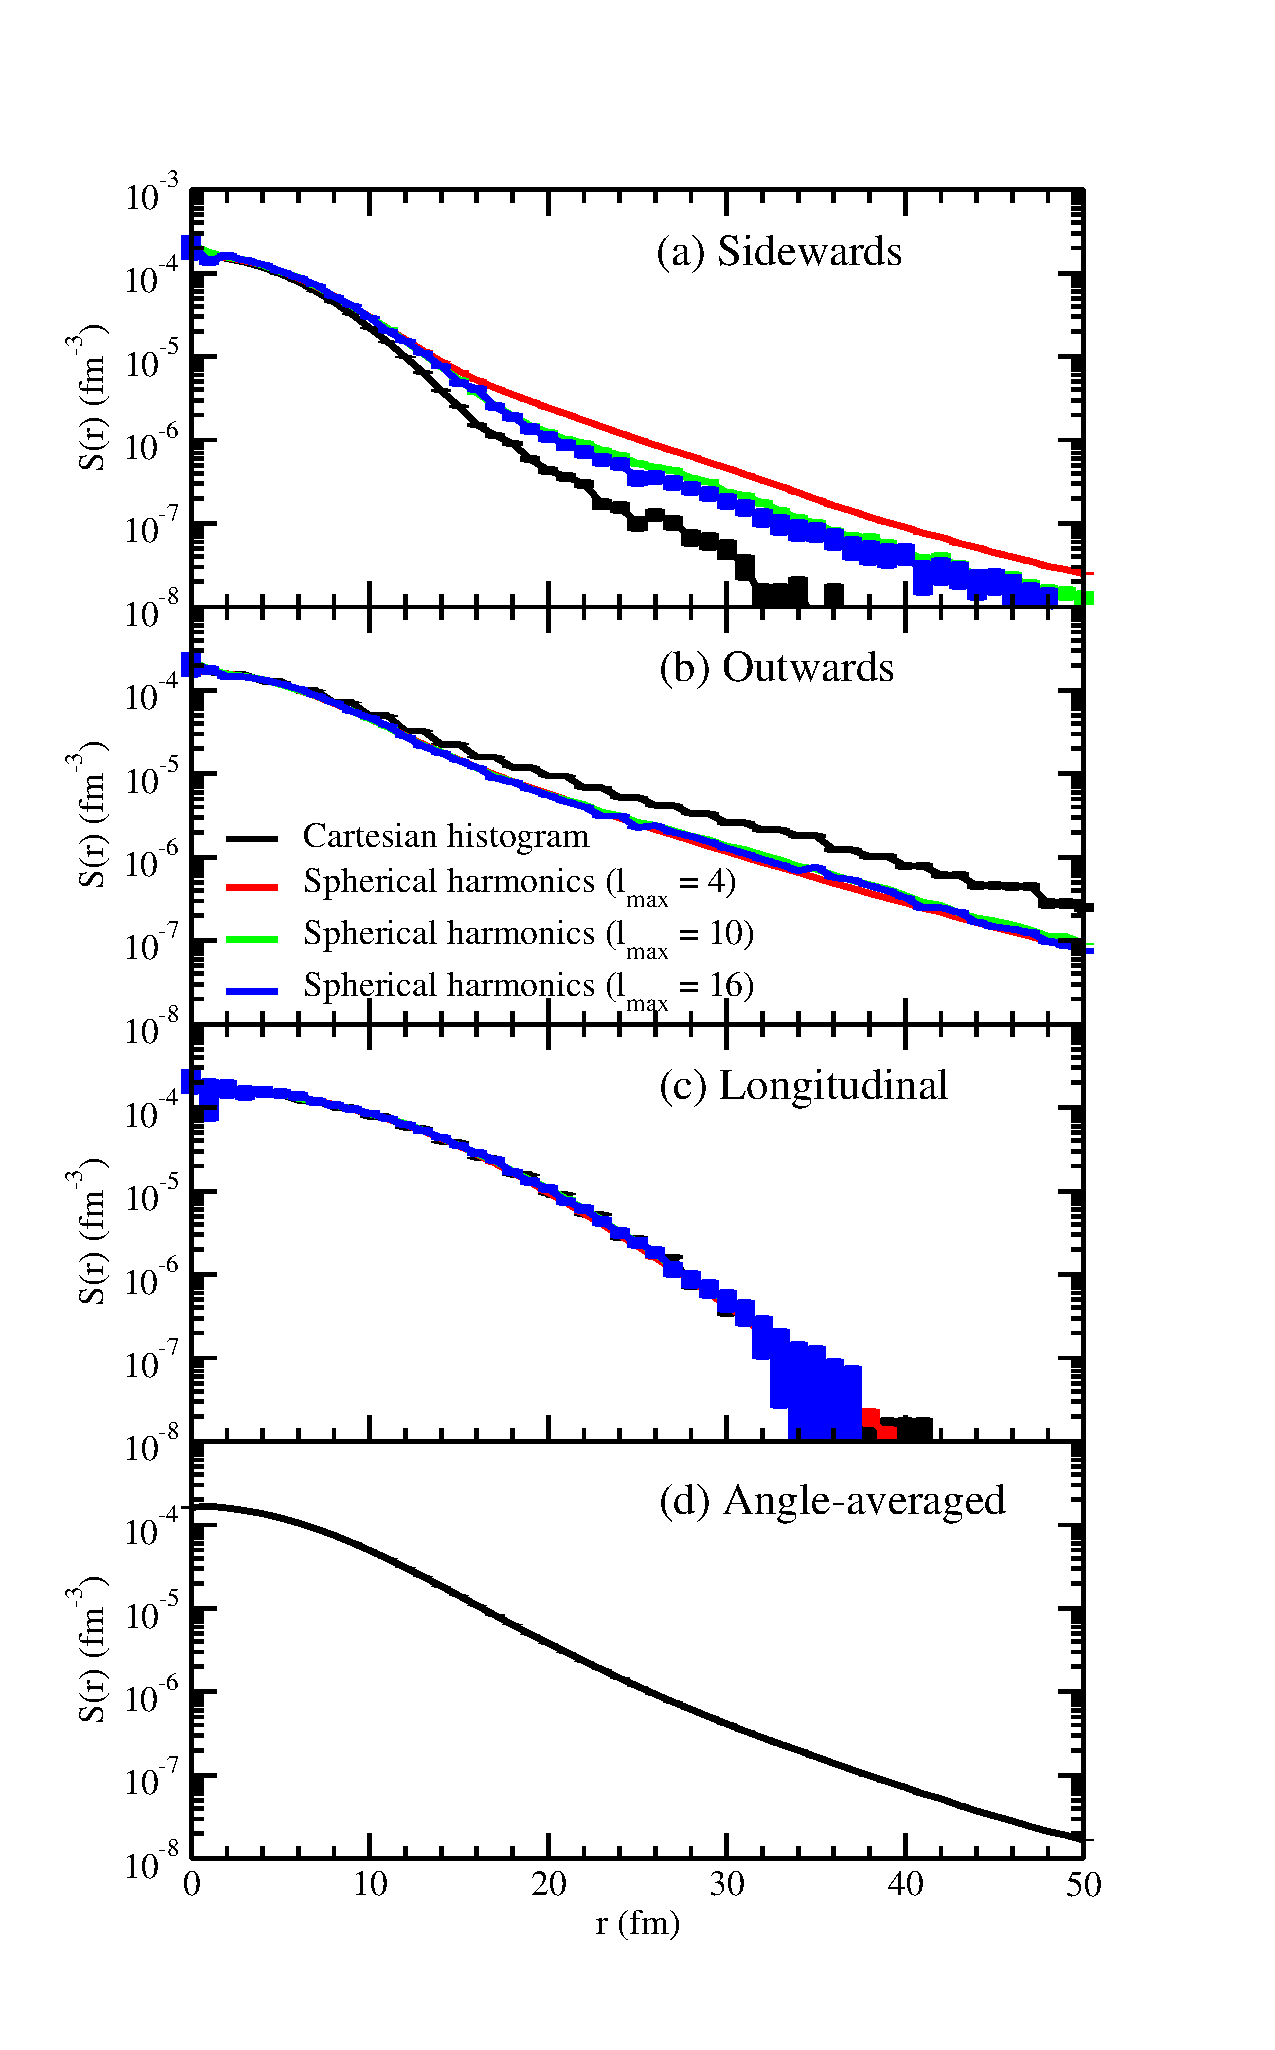
\includegraphics[width=0.47\textwidth]{chum_source_4panel}    
\caption{\label{corrTailSlice} slices of the correlation  we obtain folding our test source with a non-interacting like-pion kernel, a $\pi^{+}\pi^{+}$  and a $K^{+}K^{+}$ kernel}    
\end{figure}

\begin{figure}
%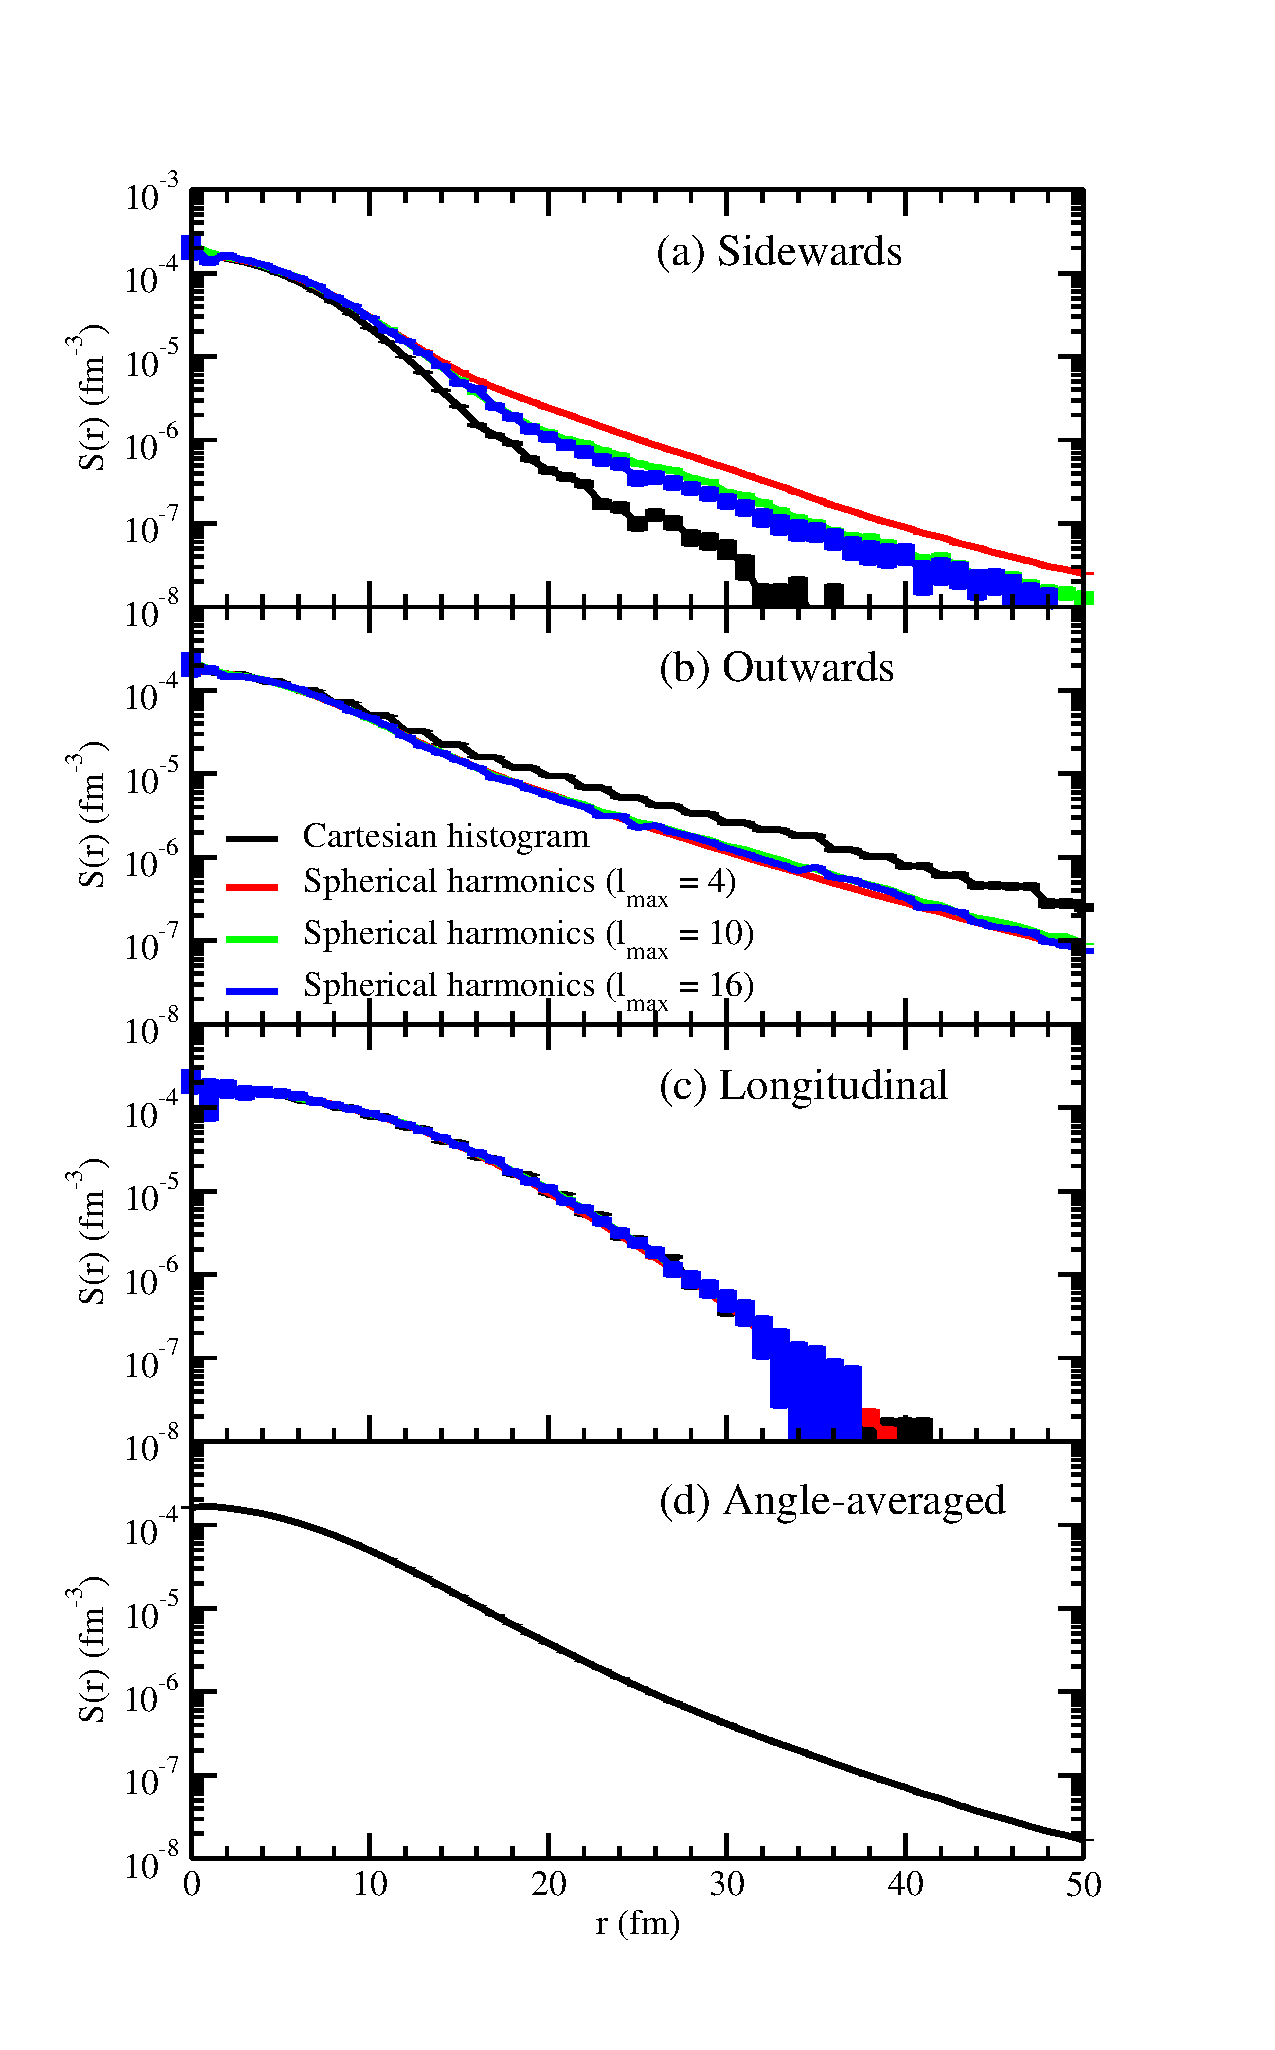
\includegraphics[width=0.47\textwidth]{chum_source_4panel}    
\caption{\label{corrTailTerm} spherical harmonic terms of the correlation  we obtain folding our test source with a non-interacting like-pion kernel, a $\pi^{+}\pi^{+}$  and a $K^{+}K^{+}$ kernel}    
\end{figure}

\section{Imaging analysis of the test correlations in the various bases}    

%-------------------------------------------
\section*{Acknowledgements}
%-------------------------------------------
This work was performed under the auspices of the U.S. Department of Energy by Lawrence Livermore National  Laboratory under Contract W-7405-Eng-48.  
\nobreak

%-------------------------------------------
\begin{thebibliography}{70}
%-------------------------------------------
%generic citing {\it et al.}, Phys. Rev. Lett. {\bf 00}:00000 (2000)
%% GGLP and HBT
\bibitem{gol60}G. Goldhaber {\em et al.}, Phys. Rev. {\bf 120}, 300 (1960).
\bibitem{hbt54}R.~Hanbury-Brown and R.~Twiss, Phil.~Mag. {\bf 45}:663, (1954).
%%Annual Review
\bibitem{annrev}M.A. Lisa, S. Pratt, R.A. Soltz, U. Wiedemann, Phys. Rev. Lett. {\bf 55}:357 (2005).
%% imaging and ppg052
\bibitem{imag1}D.A. Brown and P.~Danielewicz, Phys.~Lett.~B {\bf 398}, 252 (1997).
\bibitem{imag2}D.A. Brown and P.~Danielewicz, Phys.~Rev.~C {\bf 57}, 2474 (1998).
\bibitem{imag3}D.A. Brown and P.~Danielewicz, Phys. Rev.~C {\bf 64}, 014902 (2001).
\bibitem{ppg052}S. Adler {\it et al.}, Phys. Rev. Lett., {\bf 98}:132301 (2007).
\bibitem{makeclm}A. Kisiel and D.A. Brown, submitted to Phys. Rev.~C (2009).
%% Ron's review paper
\bibitem{3dimaging}D. Brown \etal\ Phys. Rev. C {\bf 72}: 054902 (2005).
%% Pratt et al two-pion correlations (a BP coord ref)
\bibitem{pratt_90}S.~Pratt, T.~Cs{\"o}rg\H{o} and J.~Zim\'{a}nyi, Phys. Rev.~C {\bf 42}, 2646 (1990). 
%%K-P eqn
\bibitem{koonin_77}S.E.~Koonin, Phys. Lett. {\bf B70}, 43 (1977).
%% Panitkin-Brown paper
\bibitem{panitkin_99_1} S.Y.~Panitkin and D.A.~Brown, Phys.~Rev.~C {\bf 61}, 021901(R) (1999).
%% Wiedemann, Resonance contributions to HBT correlation radii}
\bibitem{Wiedemann:1996ig} U.A.~Wiedemann, and U.W. Heinz, Phys.~Rev.~C,{\bf 56}, 3256 (1997).
\bibitem{Sullivan93}J. Sullivan  {\it et al.}, Phys. Rev. Lett. {\bf 70}:3000 (1993).
\bibitem{srcTail} D. A. Brown, R. Soltz, J. Newby, A. Kisiel, Phys. Rev. C {76}, 044906 (2007).     
%% Blast-wave
\bibitem{blastwave}F. Reti\`{e}re and M.A. Lisa, Phys. Rev. C {\bf 70}, 044907 (2004).
\end{thebibliography}

%=============================================================================
%  "EndMatter"
%=============================================================================

\end{document}
